
The TFHE scheme is designed for homomorphic addition and multiplication on integers (especially bit-wise computation, like logic circuits). Unlike BFV, GBV, or CKKS, TFHE is characterized by fast noise bootstrapping; therefore, it is efficient for processing deep multiplication depths. TFHE's noise bootstrapping technique can be further applied to functional encryption.

In TFHE, each plaintext is encrypted as an LWE ciphertext. Therefore, TFHE's ciphertext-to-ciphertext addition, ciphertext-to-plaintext addition, and ciphertext-to-plaintext multiplication are implemented based on GLWE's homomorphic addition and multiplication described in $\autoref{part:generic-fhe}$, with $n = 1$ to make GLWE an LWE.

This section will explain TFHE's novel components: key switching, ciphertext-to-ciphertext multiplication, coefficient extraction, and noise bootstrapping. 

$ $

\begin{tcolorbox}[
    title = \textbf{Required Background},    % box title
    colback = white,    % light background; tweak to taste
    colframe = black,  % frame colour
    boxrule = 0.8pt,     % line thickness
    left = 1mm, right = 1mm, top = 1mm, bottom = 1mm % inner padding
]
\begin{itemize}
  \item \autoref{sec:modulo}: \nameref{sec:modulo}
  \item \autoref{sec:group}: \nameref{sec:group}
  \item \autoref{sec:field}: \nameref{sec:field}
  \item \autoref{sec:order}: \nameref{sec:order}
  \item \autoref{sec:polynomial-ring}: \nameref{sec:polynomial-ring}
  \item \autoref{sec:decomp}: \nameref{sec:decomp}
  \item \autoref{sec:modulus-rescaling}: \nameref{sec:modulus-rescaling}
  \item \autoref{sec:lattice}: \nameref{sec:lattice}
  \item \autoref{sec:lwe}: \nameref{sec:lwe}
  \item \autoref{sec:rlwe}: \nameref{sec:rlwe}
  \item \autoref{sec:glwe}: \nameref{sec:glwe}
  \item \autoref{sec:glev}: \nameref{sec:glev}
  \item \autoref{sec:ggsw}: \nameref{sec:ggsw}
  \item \autoref{sec:glwe-add-cipher}: \nameref{sec:glwe-add-cipher}
  \item \autoref{sec:glwe-add-plain}: \nameref{sec:glwe-add-plain}
  \item \autoref{sec:glwe-mult-plain}: \nameref{sec:glwe-mult-plain}
  \item \autoref{subsec:modulus-switch-lwe}: \nameref{subsec:modulus-switch-lwe}
  \item \autoref{sec:glwe-key-switching}: \nameref{sec:glwe-key-switching}
\end{itemize}
\end{tcolorbox}

\clearpage

\subsection{Encryption and Decryption}
\label{subsec:tfhe-enc-dec}

TFHE encrypts and decrypts ciphertexts based on the LWE cryptosystem (\autoref{sec:lwe}), which is equivalent to the GLWE cryptosystem (\autoref{sec:glwe}) with $n = 1$.


\begin{tcolorbox}[title={\textbf{\tboxlabel{\ref*{subsec:tfhe-enc-dec}} TFHE Encryption and Decryption}}]
\textbf{\underline{Initial Setup}:} $\Delta = \dfrac{q}{t}$, $\vec{s} \xleftarrow{\$} \mathbb{Z}_2^k$  \textcolor{red}{\# where $t$ divides $q$, and each element of $\vec{s}$ is a 0-degree polynomial}

$ $

\par\noindent\rule{\textwidth}{0.4pt}

\textbf{\underline{Encryption Input}:} $m \in \mathbb{Z}_t$, $\vec{a} \xleftarrow{\$} \mathbb{Z}_q^k$, $e \xleftarrow{\chi_\sigma} \mathbb{Z}_q$ \textcolor{red}{\# each element of $\vec{a}$ is a 0-degree polynomial}
\begin{enumerate}
\item Scale up $m \longrightarrow \Delta \cdot m \text{ } \in \mathbb{Z}_q$

\item Compute $b = \vec{a} \cdot \vec{s} + \Delta  m + e \text{ } \bmod q$
\item $\textsf{LWE}_{\vec{s},\sigma}(\Delta  m) = (\vec{a}, b) \text{ } \in \mathbb{Z}_q^{k + 1}$ 
\end{enumerate}

\par\noindent\rule{\textwidth}{0.4pt}

\textbf{\underline{Decryption Input}:} $\textsf{ct} = (\vec{a}, b) \text{ } \in \mathbb{Z}_q^{k+1}$
\begin{enumerate}
\item $\textsf{LWE}^{-1}_{\vec{s},\sigma}(\textsf{ct}) = b - \vec{a}\cdot \vec{s} = \Delta  m + e  \pmod q$

\item Scale down $\Bigg\lceil\dfrac{ \Delta  m + e } {\Delta}\Bigg\rfloor = m \text{ } \in \mathbb{Z}_t$ \textcolor{red}{ \# i.e., modulus switch from $q \rightarrow t$}
\end{enumerate}

$ $

\textbf{{Condition for Correct Decryption}:}
\begin{itemize}
\item The noise $e$ grown over homomorphic operations should be: $e < \dfrac{\Delta}{2}$. 
\end{itemize}

\end{tcolorbox}

\subsection{Homomorphic Ciphertext-to-Ciphertext Addition}
\label{subsec:tfhe-add-cipher}

TFHE's ciphertext-to-ciphertext addition uses LWE's ciphertext-to-ciphertext addition scheme, which is equivalent to GLWE's ciphertext-to-ciphertext addition scheme (\autoref{sec:glwe-add-cipher}) with $n = 1$.  


\begin{tcolorbox}[title={\textbf{\tboxlabel{\ref*{subsec:tfhe-add-cipher}} TFHE Ciphertext-to-Ciphertext Addition}}]
$\textsf{LWE}_{\vec{s}, \sigma}(\Delta m^{\langle 1 \rangle} ) + \textsf{LWE}_{\vec{s}, \sigma}(\Delta m^{\langle 2 \rangle} ) $

$ = ( \vec{a}^{\langle 1 \rangle}, \text{ } b^{\langle 1 \rangle}) + (\vec{a}^{\langle 2 \rangle}, \text{ } b^{\langle 2 \rangle}) $

$ = ( \vec{a}^{\langle 1 \rangle} + \vec{a}^{\langle 2 \rangle}, \text{ } b^{\langle 1 \rangle} + b^{\langle 2 \rangle} ) $

$= \textsf{LWE}_{\vec{s}, \sigma}(\Delta(m^{\langle 1 \rangle} + m^{\langle 2 \rangle}) )$
\label{Here}
\end{tcolorbox}


\subsection{Homomorphic Ciphertext-to-Plaintext Addition}
\label{subsec:tfhe-add-plain}

TFHE's ciphertext-to-plaintext addition (where $\lambda$ is a constant to add) uses LWE's ciphertext-to-plaintext addition scheme, which is equivalent to GLWE's ciphertext-to-plaintext addition scheme (\autoref{sec:glwe-add-plain}) with $n = 1$.  

\begin{tcolorbox}[title={\textbf{\tboxlabel{\ref*{subsec:tfhe-add-plain}} TFHE Ciphertext-to-Plaintext Addition}}]
$\textsf{LWE}_{\vec{s}, \sigma}(\Delta m) + \Delta \lambda $

$=  (\vec{a}, \text{ } B) + \Delta \lambda$

$=  (\vec{a}, \text{ } B + \Delta\lambda)$

$= \textsf{LWE}_{\vec{s}, \sigma}(\Delta (m + \lambda) )$
\end{tcolorbox}


\subsection{Homomorphic Ciphertext-to-Plaintext Multiplication}
\label{subsec:tfhe-mult-plain}

TFHE's ciphertext-to-plaintext multiplication uses LWE's ciphertext-to-plaintext multiplication scheme, which is equivalent to GLWE's ciphertext-to-plaintext multiplication scheme (\autoref{sec:glwe-mult-plain}) with $n = 1$.  

\begin{tcolorbox}[title={\textbf{\tboxlabel{\ref*{subsec:tfhe-mult-plain}} TFHE Ciphertext-to-Plaintext Multiplication}}]
$\textsf{LWE}_{\vec{s}, \sigma}(\Delta m) \cdot \lambda$

$= (\vec{a}, \text{ } b) \cdot \lambda$

$= (\lambda\cdot \vec{a}, \text{ } \lambda \cdot b)$

$= \textsf{LWE}_{\vec{s}, \sigma}(\Delta (m \cdot \lambda) )$
\end{tcolorbox}


\subsection{Homomorphic Key Switching}
\label{subsec:tfhe-key-switching}

\textbf{- Reference:} 
\href{https://www.zama.ai/post/tfhe-deep-dive-part-3}{TFHE Deep Dive - Part III - Key switching and leveled multiplications}~\cite{tfhe-3}

TFHE's key switching scheme changes an LWE ciphertext's the secret key from $\vec{s}$ to $\vec{s}_{'}$. This scheme is essentially LWE's key switching scheme. Specifically, this is equivalent to the alternative GLWE version's (\autoref{subsec:glwe-alternative}) key switching scheme (\autoref{sec:glwe-key-switching}) with $n = 1$ as follows:

\begin{tcolorbox}[title={\textbf{\tboxlabel{\ref*{subsec:tfhe-key-switching}} TFHE Key Switching}}]
$\textsf{LWE}_{\vec{s}_{'},\sigma}(\Delta m) = (0, b) + \bm{\langle} \textsf{Decomp}^{\beta, l}(\vec{a}), \text{ } \textsf{Lev}_{\vec{s}_{'}, \sigma}^{\beta, l}(\vec{s}) \bm{\rangle}$
\end{tcolorbox}


\subsection{Homomorphic Ciphertext-to-Ciphertext Multiplication}
\label{subsec:tfhe-mult-cipher}

\textbf{- Reference:} 
\href{https://www.zama.ai/post/tfhe-deep-dive-part-3}{TFHE Deep Dive - Part III - Key switching and leveled multiplications}~\cite{tfhe-3}

$ $

TFHE supports multiplication of two ciphertexts in the form: $\textsf{LWE}_{\vec{s}, \sigma}(\Delta m_1) \cdot \textsf{GSW}_{\vec{s}, \sigma}^{\beta, l}(m_2)$. 

$ $

\noindent The 1st term $\textsf{LWE}_{\vec{s}, \sigma}(\Delta m_1)$ comes from one of the followings: 
\begin{itemize}
\item A fresh LWE encryption (\autoref{subsec:glwe-enc}) of plaintext $m_1$. 
\item A homomorphically added result of two LWE ciphertexts (\autoref{sec:glwe-add-cipher}). 
\item A homomorphically multiplied result of a LWE ciphertext with a plaintext (\autoref{sec:glwe-mult-plain}). 
\end{itemize}

$ $

\noindent The 2nd term $\textsf{GSW}_{\vec{s}, \sigma}^{\beta, l}(m_2)$ comes from one of the followings:
\begin{itemize}
\item A fresh GSW encryption (\autoref{subsec:ggsw-enc}) of plaintext $m_2$.
\item Converted from $\textsf{LWE}_{\vec{s}, \sigma}(\Delta m_2)$ into $\textsf{GSW}_{\vec{s}, \sigma}^{\beta, l}(m_2)$ by \textit{circuit bootstrapping} (this will be covered in the future).
\end{itemize}

$ $

\noindent Remember the followings: 

$\textsf{LWE}_{\vec{s}, \sigma}(\Delta m_1) = (\vec{a}, b) \in \mathbb{Z}_{q}^{k + 1}$, where $b = \vec{a} \cdot \vec{s} + \Delta m_1 + e$ 

$ $

$\textsf{GSW}_{\vec{s}, \sigma}^{\beta, l}(m_2) = \Bigr \{ \{ \textsf{Lev}_{\vec{s}, \sigma}^{\beta, l} (-s_i \cdot m_2)  \}_{i=0}^{k-1}, \textsf{Lev}_{\vec{s}, \sigma}^{\beta, l}(m_2) \Bigl \} \in \mathbb{Z}_{q }^{(k-1) \cdot l \cdot (k-1)}$ \textcolor{red}{\# from \autoref{subsec:ggsw-enc}}

$ $

\noindent Let's use the following notations:

$\textsf{GSW}_{\vec{s}, \sigma}^{\beta, l}(m_2) = {\bar{\textsf{ct}}} = (\bar{\textsf{ct}}_0,. \bar{\textsf{ct}}_1, \gap{$\cdots$} \bar{\textsf{ct}}_k)$ 

$\bar{\textsf{ct}}_i = \textsf{Lev}_{\vec{s}, \sigma}^{\beta, l}(-s_i \cdot m_2)$ for $0 \leq i \leq (k-1)$

$\bar{\textsf{ct}}_k = \textsf{Lev}_{\vec{s}, \sigma}^{\beta, l}(m_2)$

$\textsf{ct} = \textsf{LWE}_{\vec{s}, \sigma}(\Delta m_1) = (\vec{a}, b) = (a_0, a_1, \gap{$\cdots$}, a_{k-1}, b) = (\textsf{ct}_0, \textsf{ct}_1, \cdots, \textsf{ct}_k)$

$ $

\noindent Let's define the following TFHE ciphertext multiplication operation: 

$\textsf{ct} \cdot {\bar{\textsf{ct}}} = \sum\limits_{i=0}^{k}\langle \textsf{Decomp}^{\beta, l}(\textsf{ct}_i), \bar{\textsf{ct}}_i \rangle$

$ $

\noindent Then, the following is true:

\begin{tcolorbox}[title={\textbf{\tboxlabel{\ref*{subsec:tfhe-mult-cipher}} TFHE Ciphertext-to-Ciphertext Multiplication}}]
$\textsf{ct} = \textsf{LWE}_{\vec{s}, \sigma}(\Delta m_1) = (a_0, a_1, \cdots, a_{k-1}, b)$

$\bar{C} = \textsf{GSW}_{\vec{s}, \sigma}^{\beta, l}(m_2) = \bm( \textsf{Lev}_{\vec{s}, \sigma}(-s_0\cdot m_2), \textsf{Lev}_{\vec{s}, \sigma}^{\beta, l}(-s_1\cdot m_2), \cdots, \textsf{Lev}_{\vec{s}, \sigma}^{\beta, l}(-s_{k-1}\cdot m_2), \textsf{Lev}_{\vec{s}, \sigma}^{\beta, l}(m_2)  \bm)$

$\textsf{LWE}_{\vec{s}, \sigma}(\Delta m_1) \cdot \textsf{GSW}_{\vec{s}, \sigma}^{\beta, l}(m_2) = \sum\limits_{i=0}^{k}\langle \textsf{Decomp}^{\beta, l}(\textsf{ct}_i), \bar{C}_i \rangle = \textsf{LWE}_{\vec{s}, \sigma}(\Delta m_1 m_2)$
\end{tcolorbox}

This means that multiplying two TFHE ciphertexts (one is in LWE and another in GSW) and decrypting the resulting LWE ciphertext gives the same result as multiplying their two original plaintexts. 

$ $

\textbf{\underline{Proof}}
\begin{enumerate}
\item $\sum\limits_{i=0}^{k}\langle \textsf{Decomp}^{\beta, l}(\textsf{ct}_i), \bar{\textsf{ct}}_i \rangle$ \\
$= \langle \textsf{Decomp}^{\beta, l}(a_0), \bar{\textsf{ct}}_0 \rangle + \langle \textsf{Decomp}^{\beta, l}(a_1), \bar{\textsf{ct}}_1 \rangle + \gap{$\cdots$} + \langle \textsf{Decomp}^{\beta, l}(a_{k-1}), \bar{\textsf{ct}}_{k-1} \rangle + \langle \textsf{Decomp}^{\beta, l}(b), \bar{\textsf{ct}}_k \rangle$ \\
\textcolor{red}{\# expanding the dot product of two vectors}
\item For $i = k$: \\
$\textsf{Decomp}^{\beta, l}(b) = (b_1, b_2, \gap{$\cdots$}, b_l)$, where $b = b_1\dfrac{q}{\beta^1} + b_2\dfrac{q}{\beta^2} + \gap{$\cdots$} + b_l\dfrac{q}{\beta^l}$ \textcolor{red}{\# from \autoref{subsec:poly-decomp}}\\
$\bar{\textsf{ct}}_k = \textsf{Lev}_{\vec{s}, \sigma}^{\beta, l}(m_2) = \left(\textsf{LWE}_{\vec{s}, \sigma}\left(m_{2}\dfrac{q}{\beta^1}\right), \textsf{LWE}_{\vec{s}, \sigma}\left(m_{2}\dfrac{q}{\beta^2}\right), \gap{$\cdots$}, \textsf{LWE}_{\vec{s}, \sigma}\left(m_{2}\dfrac{q}{\beta^l}\right) \right)$ \\
$ $

Therefore: \\
$\langle \textsf{Decomp}^{\beta, l}(b), \bar{\textsf{ct}}_k \rangle$\\
$= b_1 \cdot \textsf{LWE}_{\vec{s}, \sigma} \left (m_{2}\dfrac{q}{\beta^1} \right ) + b_2 \cdot \textsf{LWE}_{\vec{s}, \sigma} \left (m_{2}\dfrac{q}{\beta^2} \right ) + \gap{$\cdots$} + b_l \cdot \textsf{LWE}_{\vec{s}, \sigma} \left (m_{2}\dfrac{q}{\beta^l}\right)$ \\
$= \textsf{LWE}_{\vec{s}, \sigma} \left (b_1m_{2}\dfrac{q}{\beta^1} \right ) + \textsf{LWE}_{\vec{s}, \sigma} \left (b_2m_{2}\dfrac{q}{\beta^2} \right ) + \gap{$\cdots$} + \textsf{LWE}_{\vec{s}, \sigma} \left (b_lm_{2}\dfrac{q}{\beta^l}\right)$ \textcolor{red}{\# from \autoref{sec:glwe-mult-plain}} \\
$= \textsf{LWE}_{\vec{s}, \sigma} \left (b_1m_{2}\dfrac{q}{\beta^1} + b_2m_{2}\dfrac{q}{\beta^2} + \gap{$\cdots$} + b_lm_{2}\dfrac{q}{\beta^l}\right)$ \textcolor{red}{\# from \autoref{sec:glwe-add-cipher}}\\
$= \textsf{LWE}_{\vec{s}, \sigma} \left (m_{2} \cdot \left ( b_1\dfrac{q}{\beta^1} + b_2\dfrac{q}{\beta^2} + \gap{$\cdots$} + b_l\dfrac{q}{\beta^l} \right)\right)$ \\
$= \textsf{LWE}_{\vec{s}, \sigma} (m_{2}b)$ \textcolor{red}{\# from \autoref{subsec:poly-decomp}}

\item For $0 \leq i \leq (k - 1)$: \\
$\textsf{Decomp}^{\beta, l}(a_i) = (a_{\langle i, 1 \rangle}, a_{\langle i, 2 \rangle}, \gap{$\cdots$}, a_{\langle i, l \rangle})$, where $a_i = a_{\langle i, 1 \rangle}\dfrac{q}{\beta^1} + a_{\langle i, 2 \rangle}\dfrac{q}{\beta^2} + \gap{$\cdots$} + a_{\langle i, l \rangle}\dfrac{q}{\beta^l}$ \\
$\bar{\textsf{ct}}_i =  \textsf{Lev}_{\vec{s}, \sigma}^{\beta, l}(-s_im_2) = \left(\textsf{LWE}_{\vec{s}, \sigma}\left(-s_im_2\dfrac{q}{\beta^1}\right), \textsf{LWE}_{\vec{s}, \sigma}\left(-s_im_2\dfrac{q}{\beta^2}\right), \gap{$\cdots$}, \textsf{LWE}_{\vec{s}, \sigma}\left(-s_im_2\dfrac{q}{\beta^l}\right) \right)$ \\

$ $
Therefore: \\
$\langle \textsf{Decomp}^{\beta, l}(a_0), \bar{\textsf{ct}}_0 \rangle + \langle \textsf{Decomp}^{\beta, l}(a_1), \bar{\textsf{ct}}_1 \rangle + \gap{$\cdots$} + \langle \textsf{Decomp}^{\beta, l}(a_{k-1}), \bar{\textsf{ct}}_{k-1} \rangle$ \\
$= \sum\limits_{i=0}^{k-1}\langle \textsf{Decomp}^{\beta, l}(a_i), \bar{\textsf{ct}}_i \rangle$ \\
$= \sum\limits_{i=0}^{k-1}\left(a_{\langle i, 1\rangle} \cdot \textsf{LWE}_{\vec{s}, \sigma}\left(-s_im_2\dfrac{q}{\beta^1}\right) + a_{\langle i, 2\rangle} \cdot \textsf{LWE}_{\vec{s}, \sigma}\left(-s_im_2\dfrac{q}{\beta^2}\right) + \gap{$\cdots$} + a_{\langle i, l\rangle} \cdot \textsf{LWE}_{\vec{s}, \sigma}\left(-s_im_2\dfrac{q}{\beta^l}\right)\right)$ \\
$= \sum\limits_{i=0}^{k-1}\left(\textsf{LWE}_{\vec{s}, \sigma}\left(-a_{\langle i, 1\rangle}s_im_2\dfrac{q}{\beta^1}\right) + \textsf{LWE}_{\vec{s}, \sigma}\left(-a_{\langle i, 2\rangle}s_im_2\dfrac{q}{\beta^2}\right) + \gap{$\cdots$} + \textsf{LWE}_{\vec{s}, \sigma}\left(-a_{\langle i, l\rangle}s_im_2\dfrac{q}{\beta^l}\right)\right)$ \\
$= \sum\limits_{i=0}^{k-1}\textsf{LWE}_{\vec{s}, \sigma}\left(-a_{\langle i, 1\rangle}s_im_2\dfrac{q}{\beta^1} + -a_{\langle i, 2\rangle}s_im_2\dfrac{q}{\beta^2} + \gap{$\cdots$} + -a_{\langle i, l\rangle}s_im_2\dfrac{q}{\beta^l}\right)$ \\
$= \sum\limits_{i=0}^{k-1}\textsf{LWE}_{\vec{s}, \sigma}\left(-s_im_2 \cdot \left(a_{\langle i, 1\rangle}\dfrac{q}{\beta^1} + a_{\langle i, 2\rangle}\dfrac{q}{\beta^2} + \gap{$\cdots$} + a_{\langle i, l\rangle}\dfrac{q}{\beta^l}\right)\right)$ \\
$= \sum\limits_{i=0}^{k-1}\textsf{LWE}_{\vec{s}, \sigma}(-s_im_2a_i)$
\item According to step 2 and 3, \\
$\sum\limits_{i=0}^{k}\langle \textsf{Decomp}^{\beta, l}(\textsf{ct}_i), \bar{\textsf{ct}}_i \rangle$ \\
$= \sum\limits_{i=0}^{k-1}\textsf{LWE}_{\vec{s}, \sigma}(-s_im_2a_i) + \textsf{LWE}_{\vec{s}, \sigma} (m_{2}b)$ \\ 
$= \textsf{LWE}_{\vec{s}, \sigma}\Big(\sum\limits_{i=0}^{k-1}(-s_im_2a_i) + m_{2}b\Big)$ \textcolor{red}{\# addition of two GLWE ciphertexts} \\ 
$= \textsf{LWE}_{\vec{s}, \sigma}\Big(m_2b - \sum\limits_{i=0}^{k-1}m_2a_is_i\Big)$  \\ 
$= \textsf{LWE}_{\vec{s}, \sigma}\Big(m_2(b - \sum\limits_{i=0}^{k-1}a_is_i)\Big)$\\
$= \textsf{LWE}_{\vec{s}, \sigma}(m_2(\Delta m_1 + e))$ \\
$= \textsf{LWE}_{\vec{s}, \sigma}(\Delta m_1m_2 + m_2e)$ \\
$\approx \textsf{LWE}_{\vec{s}, \sigma}(\Delta m_1m_2)$ \textcolor{red}{\# given $e$ is small and thus $m_2e$ is also small}
\end{enumerate}

\subsubsection{Discussion on the Noise Growth}

Note that after ciphertext-to-ciphertext multiplication, the noise grows to: 

$ $

$\textsf{LWE}_{\vec{s}, \sigma}(\Delta m_1) \cdot \textsf{GSW}_{S, \sigma}^{\beta, l}(m_2) = \textsf{LWE}_{\vec{s}, \sigma}(\Delta m_1m_2 + m_2e) \text{ } (\approx \textsf{LWE}_{\vec{s}, \sigma}(\Delta m_1m_2))$

$ $

\noindent 
%This issue of noise growth is similar to that in ciphertext-to-plaintext multiplication (\autoref{subsubsec:glwe-mult-plain-discussion}). 
To reduce the noise, noise bootstrapping is needed (will be discussed in \autoref{subsec:tfhe-noise-bootstrapping}).

\subsubsection{Generalization to GLWE-to-GGSW Multiplication}
\label{subsubsec:tfhe-glwe-to-ggsw-multiplication}

We can further generalize TFHE's LWE-to-GSW multiplication to GLWE-to-GGSW multiplication between the following two ciphertexts: $\textsf{GLWE}_{\vec{S}, \sigma}(\Delta M_1) \cdot \textsf{GGSW}_{\vec{S}, \sigma}^{\beta, l}(M_2)$, where $M_1$, $M_2$, and $S$ are $(n-1)$-degree polynomials. 


$ $

\noindent The 1st term $\textsf{GLWE}_{\vec{S}, \sigma}(\Delta M_1)$ comes from one of the followings: 
\begin{itemize}
\item A fresh GLWE encryption (\autoref{subsec:glwe-enc}) of plaintext $M_1$. 
\item A homomorphically added result of two GLWE ciphertexts (\autoref{sec:glwe-add-cipher}). 
\item A homomorphically multiplied result of a GLWE ciphertext with a plaintext (\autoref{sec:glwe-mult-plain}). 
\end{itemize}

$ $

\noindent The 2nd term $\textsf{GGSW}_{\vec{S}, \sigma}^{\beta, l}(M_2)$ comes from one of the followings:
\begin{itemize}
\item A fresh GGSW encryption (\autoref{subsec:ggsw-enc}) of plaintext $M_2$.
\item Converted from $\textsf{GLWE}_{\vec{S}, \sigma}(\Delta M_2)$ into $\textsf{GGSW}_{\vec{S}, \sigma}^{\beta, l}(M_2)$ by \textit{circuit bootstrapping} (this will be covered in the future).
\end{itemize}

$ $

\noindent Remember the followings: 

$\textsf{GLWE}_{\vec{S}, \sigma}(\Delta M_1) = (A_0, A_0, \gap{$\cdots$}, A_{k-1}, B) \in \mathcal{R}_{n, q}^{k + 1}$, where $B = \sum\limits_{i=0}^{k-1}(A_i \cdot S_i) + \Delta M_1 + E$ \\ \textcolor{red}{\# from \autoref{subsec:glwe-enc}} 

$ $

$\textsf{GGSW}_{\vec{S}, \sigma}^{\beta, l}(M_2) = \Bigr \{ \{ \textsf{GLev}_{\vec{S}, \sigma}^{\beta, l} (-S_i \cdot M_2)  \}_{i=0}^{k-1}, \textsf{GLev}_{\vec{S}, \sigma}^{\beta, l}(M_2) \Bigl \} \in \mathcal{R}_{\langle n, q \rangle }^{(k-1) \cdot l \cdot (k-1)}$ \textcolor{red}{\# from \autoref{subsec:ggsw-enc}}

$ $

\noindent Let's use the following notations:

$\textsf{GGSW}_{\vec{S}, \sigma}^{\beta, l}(M_2) = {\bar{C}} = (\bar{C_0},. \bar{C_1}, \gap{$\cdots$} \bar{C_k})$ 

$\bar{C_i} = \textsf{GLev}_{\vec{S}, \sigma}^{\beta, l}(-S_i \cdot M_2)$ for $0 \leq i \leq (k-1)$

$\bar{C_k} = \textsf{GLev}_{\vec{S}, \sigma}^{\beta, l}(M_2)$

$\textsf{ct} = \textsf{GLWE}_{\vec{S}, \sigma}(\Delta M_1) = (C_0, C_1, \gap{$\cdots$}, C_k) = (A_0, A_1, \gap{$\cdots$}, A_{k-1}, B)$

$ $

\noindent Let's define the following TFHE ciphertext multiplication operation: 

$\textsf{ct} \cdot {\bar{C}} = \sum\limits_{i=0}^{k}\langle \textsf{Decomp}^{\beta, l}(C_i), \bar{C_i} \rangle$

$ $

\noindent Then, the following is true:

\begin{tcolorbox}[title={\textbf{\tboxlabel{\ref*{subsubsec:tfhe-glwe-to-ggsw-multiplication}} Generalization to GLWE-to-GGSW Multiplication}}]
$\textsf{ct} = \textsf{GLWE}_{\vec{S}, \sigma}(\Delta M_1) = (A_0, A_1, \cdots, A_{k-1}, B)$

$\bar{C} = \textsf{GGSW}_{\vec{S}, \sigma}^{\beta, l}(M_2)$

$ = \bm(\textsf{GLev}_{\vec{S}, \sigma}^{\beta, l}(-S_0\cdot M_2), \textsf{GLev}_{\vec{S}, \sigma}^{\beta, l}(-S_1\cdot M_2), \cdots, \textsf{GLev}_{\vec{S}, \sigma}^{\beta, l}(-S_{k-1}\cdot M_2), \textsf{GLev}_{\vec{S}, \sigma}^{\beta, l}(M_2)\bm)$

$ $

$\textsf{GLWE}_{\vec{S}, \sigma}(\Delta M_1) \cdot \textsf{GGSW}_{\vec{S}, \sigma}^{\beta, l}(M_2) = \sum\limits_{i=0}^{k}\langle \textsf{Decomp}^{\beta, l}(C_i), \bar{C_i} \rangle = \textsf{GLWE}_{\vec{S}, \sigma}(\Delta M_1 M_2)$
\end{tcolorbox}

This means that multiplying two TFHE ciphertexts (one is in GLWE and another in GGSW) and decrypting the resulting GLWE ciphertext gives the same result as multiplying their two original plaintexts. 

$ $

\textbf{\underline{Proof}}
\begin{enumerate}
\item $\sum\limits_{i=0}^{k}\langle \textsf{Decomp}^{\beta, l}(C_i), \bar{C_i} \rangle$ \\
$= \langle \textsf{Decomp}^{\beta, l}(A_0), \bar{C_0} \rangle + \langle \textsf{Decomp}^{\beta, l}(A_1), \bar{C_1} \rangle + \gap{$\cdots$} + \langle \textsf{Decomp}^{\beta, l}(A_{k-1}), \bar{C}_{k-1} \rangle + \langle \textsf{Decomp}^{\beta, l}(B), \bar{C_k} \rangle$ \\
\textcolor{red}{\# expanding the dot product of two vectors}
\item For $i = k$: \\
$\textsf{Decomp}^{\beta, l}(B) = (B_1, B_2, \gap{$\cdots$}, B_l)$, where $B = B_1\dfrac{q}{\beta^1} + B_2\dfrac{q}{\beta^2} + \gap{$\cdots$} + B_l\dfrac{q}{\beta^l}$ \textcolor{red}{\# from \autoref{subsec:poly-decomp}}\\
$\bar{C}_k = \textsf{GLev}_{\vec{S}, \sigma}^{\beta, l}(M_2) = \left(\textsf{GLWE}_{\vec{S}, \sigma}\left(M_{2}\dfrac{q}{\beta^1}\right), \textsf{GLWE}_{\vec{S}, \sigma}\left(M_{2}\dfrac{q}{\beta^2}\right), \gap{$\cdots$}, \textsf{GLWE}_{\vec{S}, \sigma}\left(M_{2}\dfrac{q}{\beta^l}\right) \right)$ \\
$ $

Therefore: \\
$\langle \textsf{Decomp}^{\beta, l}(B), \bar{C_k} \rangle$\\
$= B_1 \cdot \textsf{GLWE}_{\vec{S}, \sigma} \left (M_{2}\dfrac{q}{\beta^1} \right ) + B_2 \cdot \textsf{GLWE}_{\vec{S}, \sigma} \left (M_{2}\dfrac{q}{\beta^2} \right ) + \gap{$\cdots$} + B_l \cdot \textsf{GLWE}_{\vec{S}, \sigma} \left (M_{2}\dfrac{q}{\beta^l}\right)$ \\
$= \textsf{GLWE}_{\vec{S}, \sigma} \left (B_1M_{2}\dfrac{q}{\beta^1} \right ) + \textsf{GLWE}_{\vec{S}, \sigma} \left (B_2M_{2}\dfrac{q}{\beta^2} \right ) + \gap{$\cdots$} + \textsf{GLWE}_{\vec{S}, \sigma} \left (B_lM_{2}\dfrac{q}{\beta^l}\right)$ \textcolor{red}{\# from \autoref{sec:glwe-mult-plain}} \\
$= \textsf{GLWE}_{\vec{S}, \sigma} \left (B_1M_{2}\dfrac{q}{\beta^1} + B_2M_{2}\dfrac{q}{\beta^2} + \gap{$\cdots$} + B_lM_{2}\dfrac{q}{\beta^l}\right)$ \textcolor{red}{\# from \autoref{sec:glwe-add-cipher}}\\
$= \textsf{GLWE}_{\vec{S}, \sigma} \left (M_{2} \cdot \left ( B_1\dfrac{q}{\beta^1} + B_2\dfrac{q}{\beta^2} + \gap{$\cdots$} + B_l\dfrac{q}{\beta^l} \right)\right)$ \\
$= \textsf{GLWE}_{\vec{S}, \sigma} (M_{2}B)$ \textcolor{red}{\# from \autoref{subsec:poly-decomp}}
\item For $0 \leq i \leq (k - 1)$: \\
$\textsf{Decomp}^{\beta, l}(A_i) = (A_{\langle i, 0 \rangle}, A_{\langle i, 1 \rangle}, \gap{$\cdots$}, A_{\langle i, l \rangle})$, where $A_i = A_{\langle i, 0 \rangle}\dfrac{q}{\beta^1} + A_{\langle i, 1 \rangle}\dfrac{q}{\beta^2} + \gap{$\cdots$} + A_{\langle i, l \rangle}\dfrac{q}{\beta^l}$ \\
$\bar{C_i} =  \textsf{GLev}_{\vec{S}, \sigma}^{\beta, l}(-S_iM_2) = \left(\textsf{GLWE}_{\vec{S}, \sigma}\left(-S_iM_2\dfrac{q}{\beta^1}\right), \textsf{GLWE}_{\vec{S}, \sigma}\left(-S_iM_2\dfrac{q}{\beta^2}\right), \gap{$\cdots$}, \textsf{GLWE}_{\vec{S}, \sigma}\left(-S_iM_2\dfrac{q}{\beta^l}\right) \right)$ \\

$ $
Therefore: \\
$\langle \textsf{Decomp}^{\beta, l}(A_0), \bar{C_0} \rangle + \langle \textsf{Decomp}^{\beta, l}(A_1), \bar{C_1} \rangle + \gap{$\cdots$} + \langle \textsf{Decomp}^{\beta, l}(A_{k-1}), \bar{C}_{k-1} \rangle$ \\
$= \sum\limits_{i=0}^{k-1}\langle \textsf{Decomp}^{\beta, l}(A_i), \bar{C_i} \rangle$ \\
$= \sum\limits_{i=0}^{k-1}\left(A_{\langle i, 1\rangle} \cdot \textsf{GLWE}_{\vec{S}, \sigma}\left(-S_iM_2\dfrac{q}{\beta^1}\right) + A_{\langle i, 2\rangle} \cdot \textsf{GLWE}_{\vec{S}, \sigma}\left(-S_iM_2\dfrac{q}{\beta^2}\right) + \gap{$\cdots$} + A_{\langle i, l\rangle} \cdot \textsf{GLWE}_{\vec{S}, \sigma}\left(-S_iM_2\dfrac{q}{\beta^l}\right)\right)$ \\
$= \sum\limits_{i=0}^{k-1}\left(\textsf{GLWE}_{\vec{S}, \sigma}\left(-A_{\langle i, 1\rangle}S_iM_2\dfrac{q}{\beta^1}\right) + \textsf{GLWE}_{\vec{S}, \sigma}\left(-A_{\langle i, 2\rangle}S_iM_2\dfrac{q}{\beta^2}\right) + \gap{$\cdots$} + \textsf{GLWE}_{\vec{S}, \sigma}\left(-A_{\langle i, l\rangle}S_iM_2\dfrac{q}{\beta^l}\right)\right)$ \\
$= \sum\limits_{i=0}^{k-1}\textsf{GLWE}_{\vec{S}, \sigma}\left(-A_{\langle i, 1\rangle}S_iM_2\dfrac{q}{\beta^1} + -A_{\langle i, 2\rangle}S_iM_2\dfrac{q}{\beta^2} + \gap{$\cdots$} + -A_{\langle i, l\rangle}S_iM_2\dfrac{q}{\beta^l}\right)$ \\
$= \sum\limits_{i=0}^{k-1}\textsf{GLWE}_{\vec{S}, \sigma}\left(-S_iM_2 \cdot \left(A_{\langle i, 1\rangle}\dfrac{q}{\beta^1} + A_{\langle i, 2\rangle}\dfrac{q}{\beta^2} + \gap{$\cdots$} + A_{\langle i, l\rangle}\dfrac{q}{\beta^l}\right)\right)$ \\
$= \sum\limits_{i=0}^{k-1}\textsf{GLWE}_{\vec{S}, \sigma}(-S_iM_2A_i)$
\item According to step 2 and 3, \\
$\sum\limits_{i=0}^{k=k}\langle \textsf{Decomp}^{\beta, l}(C_i), \bar{C_i} \rangle$ \\
$= \sum\limits_{i=0}^{k-1}\textsf{GLWE}_{\vec{S}, \sigma}(-S_iM_2A_i) + \textsf{GLWE}_{\vec{S}, \sigma} (M_{2}B)$ \\ 
$= \textsf{GLWE}_{\vec{S}, \sigma}\Big(\sum\limits_{i=0}^{k-1}(-S_iM_2A_i) + M_{2}B\Big)$ \textcolor{red}{\# addition of two GLWE ciphertexts} \\ 
$= \textsf{GLWE}_{\vec{S}, \sigma}\Big(BM_2 - \sum\limits_{i=0}^{k-1}M_2A_iS_i\Big)$  \\ 
$= \textsf{GLWE}_{\vec{S}, \sigma}\Big(M_2(B - \sum\limits_{i=0}^{k-1}A_iS_i)\Big)$\\
$= \textsf{GLWE}_{\vec{S}, \sigma}(M_2(\Delta M_1 + E))$ \\
$= \textsf{GLWE}_{\vec{S}, \sigma}(\Delta M_1M_2 + M_2E)$ \\
$\approx \textsf{GLWE}_{\vec{S}, \sigma}(\Delta M_1M_2)$ \textcolor{red}{\# given $E$ is small and thus $M_2E$ is also small}
\end{enumerate}


\subsection{Coefficient Extraction}
\label{subsec:tfhe-extraction}

\textbf{- Reference:} 
\href{https://www.zama.ai/post/tfhe-deep-dive-part-4}{TFHE Deep Dive - Part IV - Programmable Bootstrapping}~\cite{tfhe-4}

$ $

In TFHE, coefficient extraction is a process of extracting a coefficient of a polynomial which is encrypted as GLWE ciphertext. The extracted coefficient is in a form of LWE ciphertext (\autoref{sec:lwe}). %We will explain how to extract the coefficient of a plaintext polynomial $M$ from a GLWE ciphertext and RLWE ciphertext, respectively. 


%\subsubsection{Coefficient Extraction from a GLWE Ciphertext}
%\label{subsubsec:tfhe-extraction-glwe}

Note that in the GLWE cryptosystem, plaintext $M$ is encoded as a polynomial, where each coefficient encodes the plaintext value $m_0, m_1, \cdots, m_{n-1}$.

%\subsubsection{Overview}
%\label{subsec:tfhe-extraction-overview}

Suppose we have a GLWE ciphertext setup as the following: \\ 
$M = \sum\limits_{j=0}^{n-1}m_jX^j \in \mathcal{R}_{\langle n, q \rangle}$ 

$S = \left(S_0 = \sum\limits_{j=0}^{n-1}s_{0,j}X^j, S_1 = \sum\limits_{j=0}^{n-1}s_{1,j}X^j, \gap{$\cdots$}, S_{k-1} = \sum\limits_{j=0}^{n-1}s_{k-1,j}X^j \right)$ 

$\textsf{GLWE}_{\vec{S}, \sigma}(\Delta M) = \left(A_0 = \sum\limits_{j=0}^{n-1}a_{0,j}X^j, A_1 = \sum\limits_{j=0}^{n-1}a_{1,j}X^j, \gap{$\cdots$}, A_{k-1} = \sum\limits_{j=0}^{n-1}a_{k-1,j}X^j, B = \sum\limits_{j=0}^{n-1}b_{j}X^j\right)$ 

$B = \sum\limits_{i=0}^{n-1}A_iS_i + \Delta M + E$ 

$E = \sum\limits_{i=0}^{n-1}e_iX^i$ 

$ $

\noindent Note that:

$\Delta M + E = B - \sum\limits_{i=0}^{n-1}A_iS_i$ 

$ = (\Delta m_0 + \Delta m_1X + \gap{$\cdots$} + \Delta m_{n-1}X^{n-1}) + (e_0 + e_1X + \gap{$\cdots$} + e_{n-1}X^{n-1})$

$= (\Delta m_0 + e_0) + (\Delta m_1 + e_1)X + \gap{$\cdots$} + (\Delta m_{n-1} + e_{n-1})X^{n-1}$

$ $

\noindent Another way to write the formula is:

$B - \sum\limits_{i=0}^{n-1}A_iS_i$ 

$ = (b_0 + b_1X + \gap{$\cdots$} + b_{n-1}X^{n-1} )$ 

$ - (a_{0,0} + a_{0,1}X + \gap{$\cdots$} + a_{0, n-1}X^{n-1})(s_{0,0} + s_{0,1}X + \gap{$\cdots$} + s_{0, n-1}X^{n-1})$ 

$ - (a_{1,0} + a_{1,1}X + \gap{$\cdots$} + a_{_1, n-1}X^{n-1})(s_{1,0} + s_{1,1}X + \gap{$\cdots$} + s_{1, n-1}X^{n-1})$ 

$ - \gap{$\cdots$} $ 

$ - (a_{k-1,0} + a_{k-1,1}X + \gap{$\cdots$} + a_{k-1, n-1}X^{n-1})(s_{k-1,0} + s_{k-1,1}X + \gap{$\cdots$} + s_{k-1, n-1}X^{n-1})$ 

$ $

$ = \left(b_0 - \left( \sum\limits_{i=0}^{k-1} \sum\limits_{j=0}^{0}(a_{i,0-j}s_{i,j}) - \sum\limits_{i=0}^{k-1} \sum\limits_{j=1}^{n-1}(a_{i,n-j}s_{i,j}) \right)\right)$

$ + \left(b_1 - \left( \sum\limits_{i=0}^{k-1} \sum\limits_{j=0}^{1}(a_{i,1-j}s_{i,j}) - \sum\limits_{i=0}^{k-1} \sum\limits_{j=2}^{n-1}(a_{i,n-j}s_{i,j})   \right) \right)\cdot X$ 



$ + \left(b_2 - \left( \sum\limits_{i=0}^{k-1} \sum\limits_{j=0}^{2}(a_{i,2-j}s_{i,j}) - \sum\limits_{i=0}^{k-1} \sum\limits_{j=3}^{n-1}(a_{i,n-j}s_{i,j})   \right) \right)\cdot X^2$ 

$ $

$\gap{$\cdots$}$ 

$ $

$ + \left(b_{n-1} - \left(  \sum\limits_{i=0}^{k-1} \sum\limits_{j=0}^{n-1}(a_{i,n-1-j}s_{i,j}) - \sum\limits_{i=0}^{k-1} \sum\limits_{j=n}^{n-1}(a_{i,n-j}s_{i,j})  \right) \right)\cdot X^{n-1}$ 

\textcolor{red}{\# Grouping the terms by same exponents}

$ $


$ $

$= \sum\limits_{h=0}^{n-1}  \left(b_h - \left(  \sum\limits_{i=0}^{k-1} \sum\limits_{j=0}^{h}(a_{i,h-j}s_{i,j}) - \sum\limits_{i=0}^{k-1} \sum\limits_{j=h+1}^{n-1}(a_{i,n+h-j}s_{i,j})  \right) \right)\cdot X^{h}  $


$ $

$= \sum\limits_{h=0}^{n-1}  C_h \cdot X^{h}  $, where $C_h = b_h - \left(  \sum\limits_{i=0}^{k-1} \sum\limits_{j=0}^{h}(a_{i,h-j}s_{i,j}) - \sum\limits_{i=0}^{k-1} \sum\limits_{j=h+1}^{n-1}(a_{i,n+h-j}s_{i,j})  \right)$

$ $

\noindent In the above $(n-1)$-degree polynomial, notice that each $X^h$ term's coefficient, $C_h$, can be expressed as an LWE ciphertext $\textsf{ct}_h$ as follows:

$S' = (s_{0,0}, s_{0,1}, \gap{$\cdots$}, s_{0,n-1}, s_{1,0}, s_{1,1}, \gap{$\cdots$}, s_{1, n-1}, \gap{$\cdots$}, s_{k-1, n-1}) = (s'_0, s'_1, \gap{$\cdots$}, s'_{nk} ) \in \mathbb{Z}_q^{nk}$


$C_h = (a'_1, a'_2, \gap{$\cdots$}, a'_{nk}, b_h) \in \mathbb{Z}_q^{nk + 1}$


\begin{figure}[h]
\[
    \text{, where } a'_{n \cdot i + j} =   
\begin{cases}
    a_{i,h - j} \text{ (if } 0 \leq j \leq h\text{)}\\
    a_{i,n + h - j} \text{ (if } h+1 \leq j \leq n-1\text{)}\\
\end{cases}
\centering , b_h \text{ is directly obtained from the polynomial } B
\]
\end{figure}

\noindent Note that $b_h - \sum\limits_{i=0}^{nk}s'_ia'_i = \Delta m_h + e_h$. This means that $C_h$ can be replaced by its encrypted version, $\textsf{LWE}_{\vec{s}_{'}, \sigma}(\Delta m_h)$, an LWE ciphertext $\textsf{ct}_h$ encrypting the $h$-th coefficient of $M$. Therefore, we just extracted $\textsf{LWE}_{\vec{s}_{'}, \sigma}(\Delta m_h)$ from $\textsf{GLWE}_{\vec{S}, \sigma}(\Delta M)$. This operation is called coefficient extraction, which does not add a noise, because it simply extracts an LWE ciphertext by reordering the polynomial of the GLWE ciphertext. 

Once we have $\textsf{LWE}_{\vec{s}_{'}, \sigma}(\Delta m_h)$, we can key-switch it from $\vec{s}_{'} \rightarrow \vec{s}$ (\autoref{subsec:tfhe-key-switching}). 

\begin{tcolorbox}[title={\textbf{\tboxlabel{\ref*{subsec:tfhe-extraction}} GLWE Ciphertext's Coefficient Extraction}}]
Given the following GLWE ciphertext: 

$M = \sum\limits_{j=0}^{n-1}m_jX^j \in \mathcal{R}_{\langle n, p \rangle}$

$\vec{S} = \left(S_0 = \sum\limits_{j=0}^{n-1}s_{0,j}X^j, S_1 = \sum\limits_{j=0}^{n-1}s_{1,j}X^j, \gap{$\cdots$}, S_{k-1} = \sum\limits_{j=0}^{n-1}s_{k-1,j}X^j \right)$

$\textsf{GLWE}_{\vec{S}, \sigma}(\Delta M) = \left(A_0 = \sum\limits_{j=0}^{n-1}a_{0,j}X^j, A_1 = \sum\limits_{j=0}^{n-1}a_{1,j}X^j, \gap{$\cdots$}, A_{k-1} = \sum\limits_{j=0}^{n-1}a_{k-1,j}X^j, B = \sum\limits_{j=0}^{n-1}b_{j}X^j\right)$

$B = \sum\limits_{i=0}^{n-1}A_iS_i + \Delta M + E \bmod q$, \text{ } $E = \sum\limits_{i=0}^{n-1}e_iX^i$

$ $

$\textsf{LWE}_{\vec{s}_{'}, \sigma}(\Delta m_h)$ is an LWE ciphertext that encrypts $\Delta M$'s $h$-th coefficient (i.e., $\Delta m_h$). $\textsf{LWE}_{\vec{s}_{'}, \sigma}(\Delta m_h)$ can be extracted from $\textsf{GLWE}_{\vec{S}, \sigma}(\Delta M)$ as follows: 

$ $

$\vec{s}_{'} = (s_{0,0}, s_{0,1}, \gap{$\cdots$}, s_{0,n-1}, s_{1,0}, s_{1,1}, \gap{$\cdots$}, s_{1, n-1}, \gap{$\cdots$}, s_{k-1, n-1}) = (s'_0, s'_1, \gap{$\cdots$}, s'_{nk} ) \in \mathbb{Z}_q^{nk}$

$\textsf{LWE}_{\vec{s}_{'}, \sigma}(\Delta m_h) = (a_0', a_1', \gap{$\cdots$} , a_{nk}', b_h) \in \mathbb{Z}_q^{nk + 1}$


\[
    \text{, where } a'_{n \cdot i + j} =   
\begin{cases}
    a_{i,h - j} \text{ (if } 0 \leq j \leq h\text{)}\\
    a_{i,n + h - j} \text{ (if } h+1 \leq j \leq n-1\text{)}\\
\end{cases}
, b_h \text{ is obtained from the polynomial } B
\]

Once we have $\textsf{LWE}_{\vec{s}_{'}, \sigma}(\Delta m_h)$, key-switch it from $\vec{s}_{'} \rightarrow \vec{s}$ (\autoref{subsec:tfhe-key-switching}).

\end{tcolorbox}



\subsection{Noise Bootstrapping}
\label{subsec:tfhe-noise-bootstrapping}


\textbf{- Reference:} 
\href{https://www.zama.ai/post/tfhe-deep-dive-part-4}{TFHE Deep Dive - Part IV - Programmable Bootstrapping}~\cite{tfhe-4}

$ $

Continuing homomorphic additions of TFHE ciphertexts does not necessarily increase the noise $e$, because $e$ is randomly generated over the Gaussian distribution, thus adding up many noises would give the mean value of 0. On the other hand, continuing homomorphic multiplications increases the noise, because the noise terms get multiplied, growing its magnitude. Thus, we need to somehow \textit{reset} the noise before it trespasses on the higher bits where plaintext $m$ resides (i.e., preventing the red noise bits from overflowing to the blue plaintext bits as shown in \autoref{fig:scaling}). The process of re-initializing the noise to a smaller value is called noise bootstrapping.

As explained in the beginning of this section, TFHE uses LWE (which is GLWE with $n = 1$) to encrypt \& decrypt a plaintext. That is, each plaintext is $m$ (a single number), encoded as a zero-degree polynomial. Further, the secret key S that encrypts each $m$ is a vector $ \{s_0, s_1, \text{ } \cdots \text{ }, s_{k-1} \}$ instead of a polynomial. On the other hand, TFHE's noise bootstrapping uses homomorphic addition between GLWE ciphertexts and homomorphic multiplication between GLWE and GGSW ciphertexts.  

%Nonetheless, the reason why we explained TFHE ciphertext addition (\autoref{subsec:glwe-add} and \autoref{subsec:glwe-add-plain}), multiplication (\autoref{subsec:tfhe-mult-cipher} and \autoref{subsec:glwe-mult-plain}), and polynomial rotation (\autoref{subsec:coeff-rotation}) in terms of GLWE is because the bootstrapping procedure we will explain in this subsection requires homomorphic addition and multiplication of GLWE ciphertexts.

Suppose we have a TFHE ciphertext as follows: 

$ $

$\textsf{LWE}_{\vec{s}, \sigma}(\Delta m) = (a_0, a_1, \gap{$\cdots$} a_{k-1}, b)$

$b = \sum\limits_{i=0}^{k-1} a_is_i + \Delta m + e_b$

$\vec{s} = (s_0, s_1, \gap{$\cdots$} s_k)$

$ $

, where $e_b$ is a big noise accumulated over a series of many ciphertext (or plaintext) multiplications. The goal of noise bootstrapping is to convert $(a_0, a_0, \gap{$\cdots$} a_{k-1}, b)$ into $(a_0', a_1', \gap{$\cdots$} a_{k-1}', b')$ such that: 

$ $

$b' = \sum\limits_{i=0}^{k-1} a_i's_i + \Delta m + e_s$

$ $

, where $e_s$ is a re-initialized noise. 

$ $
\subsubsection{Overview}
\label{subsec:bootstrapping-overview}

To implement noise bootstrapping, we create a specially designed $(n-1)$-degree polynomial $V(X)$ called a Lookup Table (LUT). The polynomial $V(X)$'s each degree term $X^{i'}$ has its exponent $i' = \Delta m_i + e$, a noisy plaintext, and its corresponding coefficient $v_{i'} = \Delta m_i$, which is a noise-free plaintext. Therefore, $V(X)$ is defined as:

$V(X) = v_0 + v_1X^1 + v_2X^2 + \gap{$\cdots$} + v_nX^{n-1}$

\text{ } $= m_0X^{\Delta m_0 + e_0} + m_0X^{\Delta m_0 + e_1} + m_0X^{\Delta m_0 + e_2} + \gap{$\cdots$} + m_0X^{\Delta m_0 + e_{\Delta - 1}}$

\text{ } $ + \text{ } m_1X^{\Delta m_1 + e_0} + m_1X^{\Delta m_1 + e_1} + m_1X^{\Delta m_1 + e_2} + \gap{$\cdots$} + m_1X^{\Delta m_1 + e_{\Delta - 1}}$

\text{ } $ + \gap{$\cdots$} $

\text{ } $ + \text{ } m_{t - 1}X^{\Delta m_{t - 1} + e_0} + m_{t - 1}X^{\Delta m_{t - 1} + e_1} + m_{t - 1}X^{\Delta m_{t - 1} + e_2} + \gap{$\cdots$} + m_{t - 1}X^{\Delta m_{t - 1} + e_{\Delta - 1}}$

$ $

We design $V$ to have the special property that its each $v_{i'}X^{i'}$ term has the special mapping of (exponent, coefficient) $= (\Delta m_i + e_{*}, m_i)$. During the TFHE setup stage, we GLWE-encrypt $V(X)$ by using our newly defined GLWE key $\vec{S}_{kb}$, a \textit{bootstrapping key}, which is different from the LWE secret key $\vec{s}$. $\vec{S}_{kb}$ is a list of $(n-1)$-degree polynomials with binary coefficients. Later, during the noise bootstrapping stage, we rotate the the coefficients of $V$ by $\Delta m + e$ positions to the left by computing $V \cdot X^{-(\Delta m + e)} = V'$, by using the polynomial coefficient rotation method 1 technique (Summary~\ref*{subsec:coeff-rotation}.1 in \autoref{subsec:coeff-rotation}). Then, we will extract the polynomial's constant term's coefficient (i.e., the left-most 0-degree term's coefficient in the rotated $V'$) by using the coefficient extraction technique (\autoref{subsec:tfhe-extraction}). Further, we will encrypt $V(X)$ as a GLWE ciphertext at the TFHE setup stage, and thus the rotated $V'(X)$'s extracted constant term's coefficient is an LWE encryption of $m$ (i.e., $\textsf{LWE}_{\vec{s}, \sigma}(\Delta m)$) with a re-initialized noise. 

To summarize, the noise bootstrapping procedure can be conceptually understood (at least for now) as follows: 

$ $

\begin{enumerate}
\item \textbf{Input:} $\textsf{LWE}_{\vec{s}, \sigma}(\Delta m + e)$ as a noisy ciphertext encrypting $m$
\item Convert the input into the form of $X^{-(\Delta m + e)}$ as a rotator of $V(X)$ (Lookup Table)
\item Rotate $V$ to the left by $\Delta m + e$ positions by computing $V \cdot X^{-(\Delta m + e)} = V'$
\item Extract the rotated $V'(X)$'s constant term's coefficient $m$ as an LWE encryption, which is $\textsf{LWE}_{\vec{s}, \sigma}(\Delta m)$
\item \textbf{Output:} $\textsf{LWE}_{\vec{s}, \sigma}(\Delta m)$ as an LWE encryption of the plaintext $m$ with a re-initialized noise. 
\end{enumerate}

$ $

The final $\textsf{LWE}_{\vec{s}, \sigma}(\Delta m)$ can be used for subsequent TFHE homomorphic operations (e.g., addition or multiplication). During this noise bootstrapping process, the polynomial $V$ is used as a \textit{dictionary} that contains the mappings from the noisy plaintext $\Delta m + e$ (i.e., as $i$ in $v_iX^i$) to the noise-free plaintext $m$ (i.e., as $v_i$ in $v_iX^i$). Therefore, $V$ is called Lookup Table (LUT). 

Then, what should be the degree of $V$? In order for $V$ to encode all possible mappings from $\Delta m + e \in \mathbb{Z}_q$ to $m \in \mathbb{Z}_t$, it should be a $(q-1)$-degree polynomial. However, $q$ is a very big number and it is computationally infeasible to manage a $(q-1)$-degree polynomial. Thus, in practice, we instead use a much smaller polynomial $V$ whose degree is $n-1$. Remember that according to our TFHE setup, $n < q$. Therefore, we need a way to \textit{compress} the big ciphertext space $\Delta m + e \in \mathbb{Z}_q$ into the smaller space $\mathbb{Z}_n$ and encode them as the exponents of $X^i$ in a \textit{proportionally} correct way. For this proportional compression from $\mathbb{Z}_q \rightarrow \mathbb{Z}_n$, we will use the LWE modulus switching technique learned from \autoref{subsec:modulus-switch-lwe}. 

\subsubsection{Modulus Switch for Noise Boootstrapping}
\label{subsec:bootstrapping-modulus-switch}

We need to compress $q$ possible plaintext elements ($\Delta m + e \in \mathbb{Z}_q$) as $n$ distinct exponents of the $(n-1)$-degree polynomial $V$, where each $v_iX^i$ term in $V$ represents a mapping from $i \rightarrow v_i$ (i.e., noisy plaintext to noise-free plaintext). However, notice that when we rotate the coefficients of the $(n-1)$-degree polynomial $V$ to the left, as $v_iX^i$ rotates around the boundary between $X^0$ and $X^{n-1}$ degree terms, $v_i$'s sign flips to $-v_i$ (as shown in the example of \autoref{subsec:coeff-rotation-ex}). Due to this coefficient sign flip, the $(n-1)$-degree polynomial $V$ can encode total $2n$ distinct coefficient states as follows: $(v_0, v_1, v_2, \gap{$\cdots$}, v_{n-1}, -v_0, -v_1, \gap{$\cdots$}, -v_{n-1})$. To move each of these $2n$ distinct coefficients to the constant term's position in $V$ (i.e., , shifting the coefficient $v_i$ to the leftmost position), the rotating computation of $V \cdot X^{-i}$ can use $2n$ distinct $i$ values, which are $\{0, 1, 2, \gap{$\cdots$}, n, n+1, \gap{$\cdots$}, 2n\}$, to move each of $(v_0, v_1, v_2, \gap{$\cdots$}, v_{n-1}, -v_0, -v_1, \gap{$\cdots$}, -v_{n-1})$ coefficients to the constant term's position. This implies that the exponent $i$ in $V\cdot X^{-i}$ can take in $2n$ distinct values to cover all possible $2n$ coefficient states. Also, remember that $i = \Delta m + e$.  Therefore, we will switch the modulo of $\Delta m + e$ from $q \rightarrow 2n$. Using the LWE modulus switching technique (\autoref{subsec:modulus-switch-lwe}), our original LWE ciphertext $\textsf{LWE}_{\vec{s}, \sigma}(\Delta m + e) = ({a}_0, {a}_1, \gap{$\cdots$} {a}_{k-1}, {b}) \in \mathbb{Z}_q^{k+1}$ (i.e., the initial input to the noise bootstrapping procedure) will be converted into the following: 

$ $

$\textsf{LWE}_{\vec{s}, \sigma}(\hat{\Delta} m) = (\hat{a}_0, \hat{a}_1, \gap{$\cdots$} \hat{a}_{k-1}, \hat{b}) \in \mathbb{Z}_{2n}^{k+1}$

$\vec{s} = (s_0, s_1, \gap{$\cdots$} s_k) \in \mathbb{Z}_2^{k+1}$  \textcolor{red}{\# the secret key stays the same, as each $s_i$ is binary}

$\hat{\Delta} = \Delta\dfrac{2n}{q} \in \mathbb{Z}_{2n}$

$\hat{a}_i = \left \lceil a_i\dfrac{2n}{q} \right \rfloor \in \mathbb{Z}_{2n}$

$\hat{e}_b = \left \lceil e_b\dfrac{2n}{q} \right \rfloor \in \mathbb{Z}_{2n}$

$\hat{b} = \left \lceil b\dfrac{2n}{q} \right \rfloor \approx \sum\limits_{i=0}^{k-1} \hat{a}_is_i + \hat{\Delta} m + \hat{e}_b  \in \mathbb{Z}_{2n}$



$ $

\para{The degree of $V(X)$ and Security}: If our goal were to design the minimal-degree polynomial $V$ whose coefficients map all possible values of the plaintext $m$, then it would be sufficient to design a ${t}$-degree polynomial $V$. Nonetheless, there are two reasons why we choose the degree of $V$ to be $2n$ instead of ${t}$: (1) greater gap of modulus switch creates more noise, due to the decreasing distance between the plaintext bits and the noise bits in the ciphertext; (2) to guarantee an enough security level-- the higher the polynomial degree $n$ is, the safer our scheme is against attacks. 



\subsubsection{Halving the Plaintext Space To be Used}
\label{subsec:tfhe-zero-padding} 

Problematically, Lookup Table $V(X)$ polynomial rotates \textit{negacyclically}, that is, $V(X)X^{n} = -V(X)$ (i.e., coefficients flip their signs with the rotating period of $n$). More generally:

\begin{figure}[h]
\[
    V(X)\cdot X^{-i}= V(X)\cdot X^{2n - i} = V(X)\cdot X^{4n - i} = \cdots = V(X)\cdot X^{-(i \gap{\text{mod} 2n)}} =  
\begin{cases}
    v_i  + v_{i+1}X + \cdots, \text{for } 0\leq i<n\\
    -v_{i} - v_{i-1}X - \cdots, \text{for } n\leq i<2n
\end{cases}
\]
\end{figure}

\noindent , where $v_i$ denotes the constant term's coefficient after rotating the polynomial $V(X)$ by $i$ positions to the left. Problematically, $v_i$ flips its sign whenever its rotation passes the boundary between $X^0$ and $X^{n-1}$. After applying modulus switch (\autoref{subsec:bootstrapping-modulus-switch}) to $V(X)$, it becomes the following polynomial:

$ $

$V(X) = v_0 + v_1X^1 + v_2X^2 + \gap{$\cdots$} + v_nX^{n-1}$

\text{ } $= m_0X^{\hat{\Delta} m_0 + \hat{e}_0} + m_0X^{\hat{\Delta} m_0 + \hat{e}_1} + m_0X^{\hat{\Delta} m_0 + \hat{e}_2} + \gap{$\cdots$} +  m_0X^{\hat{\Delta} m_0 + \hat{e}_{\hat{\Delta} - 1}}$

\text{ } $ + \text{ } m_1X^{\hat{\Delta} m_1 + \hat{e}_0} + m_1X^{\hat{\Delta} m_1 + \hat{e}_1} + m_1X^{\hat{\Delta} m_1 + \hat{e}_2} + \gap{$\cdots$} + m_1X^{\hat{\Delta} m_1 + \hat{e}_{\hat{\Delta} - 1}}$

\text{ } $ + \gap{$\cdots$} $

\text{ } $ + \text{ } m_{t - 1}X^{\hat{\Delta} m_{t - 1} + \hat{e}_0} + m_{t - 1}X^{\hat{\Delta} m_{t - 1} + \hat{e}_1} + m_{t - 1}X^{\hat{\Delta} m_{t - 1} + \hat{e}_2} + \gap{$\cdots$} + m_{t - 1}X^{\hat{\Delta} m_{t - 1} + \hat{e}_{\hat{\Delta} - 1}}$

$ $

\noindent , where $\hat{\Delta} m_{t - 1} + \hat{e}_{\hat{\Delta} - 1} \in \mathbb{Z}_{2n}$

$ $

Remember that by computing $V(X)\cdot X^{-i'}$ for  $i'= \{0, 1, \cdots , n-1\}$, we can rotate $V(X)$'s coefficients to the left by $\{0, 1, \cdots n-1 \}$ positions. Also, remember that $i' = \hat{\Delta} m_{t - 1} + \hat{e}_{\hat{\Delta} - 1}$. For each rotation of $i'= \{0, 1, \cdots , n-1\}$, we get the following values as the constant-term coefficient: 

$ $


$ $

In the above expression, $e_*$ is a noise that can range from $[0, \hat{\Delta})$. Note that all of $\hat\Delta m_i + e_0, \hat\Delta m_i + e_1, \cdots,\hat\Delta m_i + e_{\hat\Delta - 1}$ exponents are associated with the same coefficient value, $m_i$, because their underlying plaintext $m_i$ is the same. This is why the coefficients for each $m_i$ are redundantly used $\hat\Delta$ times in $V(X)$.

So far, the above sequence of $m_0, m_1, \cdots, m_{{t}/{2} - 1}$ coefficients is what we expect $V'(X)$ to return for each of $[0, n-1)$ rotations (where each $m_i < m_{i+1}$). However, the coefficient mappings all break between $[n, 2n -1)$ rotations, because their coefficients get flipped signs as they pass the term's boundary from $X^0$ to $X^{n-1}$, due to the nature of a polynomial ring modulo $(x^n + 1)$: 

$ $

$\overbrace{\overbrace{\underbrace{-m_{t/2}, -m_{t/2}, \gap{$\cdots$}}_{\text{coeff. of } X^{\hat{\Delta}m_{t/2} + e_*}}}^{\hat{\Delta} \text{ repetitions}} \overbrace{\underbrace{-m_{t/2+1}, -m_{t/2+1}, \gap{$\cdots$}}_{\text{coeff. of } X^{\hat{\Delta}m_{t/2+1} + e_*}}}^{\hat{\Delta} \text{ repetitions}} \gap{$\cdots$} \overbrace{\underbrace{-m_{t - 1}, -m_{t - 1}, \gap{$\cdots$}}_{\text{coeff. of } X^{\hat{\Delta}m_{t - 1}+ e_*} }}^{\hat{\Delta} \text{ repetitions}}}^{\text{$V(X)$'s constant term coefficient after each of $n, n+1, \cdots 2n-1$ rotations}}$ 

$ $

As you see above, the rotated $V'(X)$'s constant term coefficient shows a negacyclic pattern with the period of $n$, where the second $n$ rotation group's coefficients are the exactly negatived values of the first $n$ rotation group's values. Let's understand why this negacyclic behavior breaks the (exponent, coefficient) = $(\hat{\Delta} m + \hat e, m)$ mappings. The semantic meaning of rotating $V(X)$ to the left by 1 position means that we increase the value of $\hat{\Delta}m_i + e$ (i.e., noisy plaintext's value) by 1 when we compute $V(X)\cdot X^{\hat{\Delta}m_i + e}$, and get the rotated ${V}_{'}(X)$'s constant term coefficient $m_i$ (i.e, the mapped noise-free plaintext). Therefore, as we gradually increase the rotation count of $V$ from $[0, 2n)$, the returned $m_i$ should be a value that is either the same or greater than $m_{i-1}$, all the way to $m_{t - 1}$. This constraint holds for the first-half $i = [0, n)$, as the rotated $V'(X)$'s constant term coefficient is $m_0, \cdots, m_1, \cdots, m_{t/2 - 1}$. However, for the second-half $i = [n, 2n)$, the rotated $V'(X)$'s constant term coefficient is $-m_0, \cdots, -m_1, \cdots, -m_{t/2 - 1}$, which violates our constraint that $m_i \leq m_{i+1}$. Therefore, the combination of the first-half and the second-half domains of $i$ cannot mathematically implement a continuous modulo value range $\mathbb{Z}_t$. 

To summarize the problem, $V(X)$ cannot be used as a complete bootstrapping LUT, because it preserves the correct mappings of (exponent, coefficient) = $(\hat{\Delta} m + \hat e, m)$ only for one half of $i \in \mathbb{Z}_t$, not for the other half. 

\para{Solution:} 
Fortunately, we have verified that $V(X)$'s mappings of (exponent, coefficient) = $(\hat{\Delta} m + \hat e, \Delta m)$ preserve their consistency if $V(X)$ is rotated no more than $n-1$ positions. Therefore, the most practical solution for the negacyclic problem of polynomial rotation is to restrict $V(X)$ to be rotated no more than $n-1$ positions during the noise bootstrapping. To enforce this, we can require the TFHE application such that while it processes plaintext numbers (in its original plaintext computation logic without homomorphic computation), the application should ensure to use only some continuous $\dfrac{t}{2}$ modulo values within $\mathbb{Z}_t$. This enforces the possible values of $\hat\Delta m + \hat e$ to be continuous $n$ modulo values within $\mathbb{Z}_{2n}$. Since LUT $V(X)$ is rotated by computing $V(X)\cdot X^{-(\hat\Delta m + \hat e)}$, as we restrict $\hat\Delta m + \hat e$ to be at most $n-1$, $V(X)$ will be rotated at most $n-1$ positions during the noise bootstrapping. Thus, we can prevent the occurrences of the problematic $\{n, n+1, \gap{$\cdots$}, 2n -1 \}$ rotations that cause coefficient extraction of double-signed contradicting coefficients. 

To summarize, at the cost of halving the application's usable plaintext values to some continuous $\dfrac{t}{2}$ modulo values within $\mathbb{Z}_t$, we can prevent $V(X)$'s negacyclic rotation problem, and thereby preserve $V(X)$'s correct mappings of (exponent, coefficient) = $(\hat{\Delta} m + \hat e, \Delta m)$.

\begin{comment}
Meanwhile, the ciphertext space $q$ is unmodified, because If we take a simple example of $t = 8$, our TFHE application can design the following encoding scheme:

%Note that during the blind rotation (\autoref{subsec:bootstrapping-blind-rotation}), each step's cumulative rotation positions of the homomorphic MUX gate may end up rotating $V(X)$ more than $n$ positions. However, enforcing $0 \leq \hat\Delta m + e < n$ guarantees the rotation-finished $V'(X)$ to have the cumulative rotation count to be some integer within $[0, n) \bmod 2n$.

\begin{multicols}{2}
\begin{itemize}
 \item $0000_2 \rightarrow 000_2 (= 0)$
 \item $0001_2 \rightarrow 001_2 (= 1)$
 \item $0010_2 \rightarrow 010_2 (= 2)$
 \item $0011_2 \rightarrow 011_2 (= 3)$
 \item $0100_2 \rightarrow 100_2 (= -4)$
 \item $0101_2 \rightarrow 101_2 (= -3)$
 \item $0110_2 \rightarrow 110_2 (= 2)$
 \item $0111_2 \rightarrow 111_2 (= 1)$
\end{itemize}
\end{multicols}

By designing such binary encoding, we can encode signed integers in $\dfrac{t}{2}$ out of $t$ plaintext states (where the MSB is always 0). 
\end{comment}

Considering all these, our final LUT polynomial $V(X)$ is as follows:

\begin{tcolorbox}[title={\textbf{\tboxlabel{\ref*{subsec:tfhe-zero-padding}} Structure of Lookup Table Polynomial $\bm{V(X)}$}}]

$ $

$V(X) = v_0 + v_1X^1 + v_2X^2 + \gap{$\cdots$} + v_nX^{n-1}$

\text{ } $= m_0X^{\hat{\Delta} m_0 + \hat{e}_0} + m_0X^{\hat{\Delta} m_0 + \hat{e}_1} + m_0X^{\hat{\Delta} m_0 + \hat{e}_2} + \gap{$\cdots$} + m_0X^{\hat{\Delta} m_0 + \hat{e}_{\hat{\Delta} - 1}}$

\text{ } $ + \text{ } m_1X^{\hat{\Delta} m_1 + \hat{e}_0} + m_1X^{\hat{\Delta} m_1 + \hat{e}_1} + m_1X^{\hat{\Delta} m_1 + \hat{e}_2} + \gap{$\cdots$} + m_1X^{\hat{\Delta} m_1 + \hat{e}_{\hat{\Delta} - 1}}$

\text{ } $ + \gap{$\cdots$} $

\text{ } $ + m_{{t}/{2} - 1}X^{\hat{\Delta} m_{{t}/{2} - 1} + \hat{e}_0} + m_{{t}/{2} - 1}X^{\hat{\Delta} m_{{t}/{2} - 1} + \hat{e}_1} + m_{{t}/{2} - 1}X^{\hat{\Delta} m_{{t}/{2} - 1} + \hat{e}_2}$

\text{ } \text{ } $ + \gap{$\cdots$} + m_{{t}/{2} - 1}X^{\hat{\Delta} m_{{t}/{2} - 1} + \hat{e}_{\hat{\Delta} - 1}}$

$ $

\noindent , where $\hat\Delta = \Delta \cdot \dfrac{2n}{q}$. The application should ensure that $m_0, m_1, \cdots, m_{t/2 - 1}$ is some continuous $\dfrac{t}{2}$ modulo values in $\mathbb{Z}_t$. This constraint ensures $V(X)$'s rotation positions $\hat{\Delta} m_i + \hat e_{*}$ to be at most $n$ continuous possibilities, preventing $V(X)$ from making more than 1 full-circle rotation that triggers a negacyclic problem. 


\end{tcolorbox}


\subsubsection{Blind Rotation}
\label{subsec:bootstrapping-blind-rotation} 

Blind rotation refers to rotating an \textit{encrypted} polynomial's coefficients so that it is not possible to know how many positions the polynomial's coefficients are rotated, and after the rotation, it is not possible to see which coefficient has moved to which degree term. Blind rotation uses the basic polynomial rotation method 1 technique (Summary~\ref*{subsec:coeff-rotation} in \autoref{subsec:coeff-rotation}), with the difference that the $V(X)\cdot X^{-i}$ computation is done homomorphically. 

Note that $X^{\hat{\Delta} m + \hat{e}_b} = X^{\hat{b} - \sum_{i=0}^{k-1}{\hat{a}_is_i}}$, so we can rotate $V$ by computing $V \cdot X^{-(\hat{b} - \sum_{i=0}^{k-1}{\hat{a}_is_i})} = V \cdot X^{-\hat{b} + \sum_{i=0}^{k-1}{\hat{a}_is_i}}$. In fact, we cannot directly compute the LWE decryption formula $-\hat{b} + \sum_{i=0}^{k-1}{\hat{a}_is_i}$ (or $\hat{b} - \sum_{i=0}^{k-1}{\hat{a}_is_i}$) without the knowledge of the LWE secret key $S$. Nevertheless, there is a mathematical work-around to compute $V \cdot X^{-\hat{b} + \sum_{i=0}^{k-1}{\hat{a}_is_i}}$ without the knowledge of the secret key $S$, provided we are given $\{GGSW_{\vec{S}_{bk}, \sigma}^{\beta, l}(s_i)\}_{i=0}^{k-1}$ at the TFHE setup stage. Note that $\{GGSW_{\vec{S}_{bk}, \sigma}^{\beta, l}(s_i)\}_{i=0}^{k-1}$ is an GGSW encryption of the LWE secret key $S$, encrypted by the GLWE secret key $\vec{S}_{bk}$ (i.e., a \textit{bootstrapping} key). We use $\vec{S}_{bk}$ to homomorphically compute $V \cdot X^{-\hat{b} + \sum_{i=0}^{k-1}{\hat{a}_is_i}}$ (i.e., blindly rotate the coefficients of $V$ to the left by $\hat{b} + \sum_{i=0}^{k-1}{\hat{a}_is_i}$ positions), according to the following procedure:

\begin{enumerate}
\item GLWE-encrypt the polynomial $V$ with the bootstrapping key $\vec{S}_{bk}$ at the TFHE setup stage, so that each coefficient of $V$ gets encrypted.
\item Compute $V_0 = V \cdot X^{-\hat{b}}$, which is basically rotating $V$'s polynomials by $\hat{b}$ positions to the left. Since $\hat{b}$ is a known value visible in the LWE ciphertext, we can directly compute the rotation of $V_0 = V \cdot X^{-\hat{b}}$. 
\item Compute $V_1 = V_0 \cdot X^{\hat{a}_0s_0} = s_0 \cdot (V_0 \cdot X^{\hat{a}_0} - V_0) + V_0$.  
This formula works for the special case where $s_0 \in \{0, 1\}$: if $s_0 = 0$, then $V_1 = V_0$; else if $s_0 = 1$, then $V_1 = V_0 \cdot X^{\hat{a}_0}$. Computing $s_0 \cdot (V_0 \cdot X^{\hat{a}_0} - V_0) + V_0$ is done as a TFHE homomorphic addition and multiplication. We call this blind rotation of $V_0$, where the selection bit $s_0$ (i.e., the 1st element of the secret key vector $S$) is encrypted as a GGSW ciphertext by using $\vec{S}_{bk}$ (i.e. the bootstrapping key) and $V_0$ is an encrypted polynomial as a GLWE ciphertext. Multiplying GLWE-encrypted $V_0$ with $x^{\hat{a}_0}$ is done by GLWE ciphertext-to-plaintext multiplication (\autoref{sec:glwe-mult-plain}), and subtracting the result by GLWE-encrypted $V_0$ is done by GLWE ciphertext-to-ciphertext addition/subtraction (\autoref{sec:glwe-add-cipher}), and multiplying the result by GGSW-encrypted $s_0$ is done by GLWE-to-GGSW multiplication (\autoref{subsubsec:tfhe-glwe-to-ggsw-multiplication}), and adding the result with GLWE-encrypted $V_0$ is done by GLWE ciphertext-to-ciphertext addition. If $s_0 = 1$, then the formula's $X^{\hat{a}_0}$ term gets multiplied to $V_0$, which effectively rotates $V_0$'s coefficients by $\hat{a}_0$ positions to the right. Else if $s_0 = 0$, then $V_0$ does not get rotated and stays the same. In both cases, the resulting $V_1$ is encrypted as a new GLWE ciphertext. During this blind rotation, unless we have the knowledge of $s_0$ and $\vec{S}_{bk}$, it is impossible to know whether $V_0$ has been rotated or not, and also how many positions have been rotated.
\item By using the same blind rotation method as in the previous step, compute the GLWE encryption of $V_2 = V_1 \cdot X^{\hat{a}_1s_1} = s_1 \cdot (V_1 \cdot X^{\hat{a}}_1 - V_1) + V_1$. Note that we have the following publicly known components: $\hat{a}_1$, a GLWE encryption of $V_1$, and a GGSW ciphertext of $s_1$ encrypted by using $\vec{S}_{bk}$. 
\item Continue to compute the GLWE encryption of $V_3, V_4, \gap{$\cdots$}, V_k$ in the same manner, and we finally get a GLWE encryption of $V_k$, whose computed value is equivalent to:

$V' = V_k$

$\text{ } = V_{k-1} \cdot X^{\hat{a}_{k-1}s_{k-1}}$

$\text{ } = V_0 \cdot X^{\hat{a}_0s_0}X^{\hat{a}_1s_1}\cdots X^{\hat{a}_{k-1}s_{k-1}}$

$\text{ } = V \cdot X^{- \hat{b} + \sum_{i=0}^{k-1}{\hat{a}_is_i}} $

$\text{ } = V \cdot X^{-(\hat{\Delta} m + \hat{e}_b)}$

\end{enumerate}

This means that the GLWE encryption of the final polynomial $V_k$ will have the coefficient $m$ in its constant term, as $V(X)$ is designed to have the mapping ($\hat\Delta m + \hat e_{*}, m$).

Note that while we restrict the application's plaintext space usage to some continuous $\dfrac{t}{2}$ modulo values within $\mathbb{Z}_t$ (\autoref{subsec:tfhe-zero-padding}), this restriction does not exist in the ciphertext space. That is, it is okay for blind rotations to rotate $V(X)$ more than $n$ positions during the intermediate steps, because their invalid positions can be brought back to valid ones by their subsequent steps. Therefore, what matters for the noise bootstrapping correctness is only the completed state $V_k(X)$. The rotation-completed $V_k(X)$ must have been rotated $\hat\Delta m + \hat e$ positions to the left. Therefore, we only need to ensure that  $\hat\Delta m + \hat e$ falls within our pre-defined continuous $\dfrac{t}{2}$ modulo range within the $\mathbb{Z}_t$ domain, which is equivalent to ensuring that the aggregate rotation count is at most $n-1$ positions to avoid coefficient extraction of any double-signed contradicting coefficients. 

\begin{figure}[h!]
    \centering
  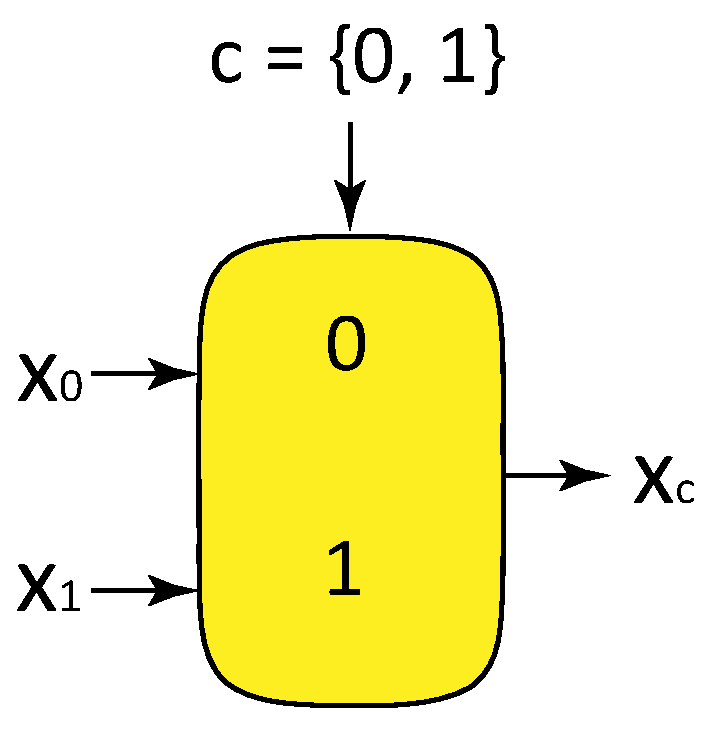
\includegraphics[width=0.2\linewidth]{figures/mux.pdf}
  \caption{An illustration of the MUX logic gate }
  \label{fig:mux}
\end{figure}

\para{Homomorphic MUX Logic Gate:} In step 3, the formula $s_0 \cdot (V_0 \cdot X^{\hat{a}_0} - V_0) + V_0$ implements the MUX logic gate as shown in \autoref{fig:mux}, where in our case $s_0$ is the selection bit that chooses between the two inputs: $V_0$ and $V_0 \cdot X^{\hat{a}_0}$. If $s_0$ is 1, then the output is $V_0 \cdot X^{\hat{a}_0}$; otherwise, the output is $V_0$. In our design, the homomorphic computation of $s_0 \cdot (V_0 \cdot X^{\hat{a}_0} - V_0) + V_0$ effectively implements a homomorphic MUX gate, where the two inputs are LWE-encrypted and the selection bit is GGSW-encrypted.


\subsubsection{Coefficient Extraction}

Finally, we use the coefficient extraction technique (\autoref{subsec:tfhe-extraction}) to extract the rotated polynomial $V'(X)$'s constant term's coefficient as an encryption of $m$: $\textsf{LWE}_{\vec{s}, \sigma}(\Delta m)$. At this point, the original $\textsf{LWE}$ ciphertext's old noise $\hat{e}_b$ has gone, and the bootstrapped new ciphertext $\textsf{LWE}_{\vec{s}, \sigma}(\Delta m)$ has a newly generated small noise $e_s$. 

In fact, the homomorphic MUX logic in the blind rotation procedure (\autoref{subsec:bootstrapping-blind-rotation}) involves lots of ciphertext multiplications and additions, which can accumulate additional noises until we reach the point of coefficient extraction. In order to limit the accumulating noises during the series of MUX logic, we can carefully adjust the security parameters. For example, we can design a narrower Gaussian distribution for sampling the noise $e$, while designing a sufficiently large $n$ to compensate for the reduced noise. Meanwhile, increasing $q$ rather makes the system less secure, because it becomes more vulnerable to Lattice reduction attacks. 






\subsubsection{Noise Bootstrapping Summary}
\label{subsec:tfhe-summary}

TFHE's noise bootstrapping procedure is summarized as follows:

\begin{tcolorbox}[title={\textbf{\tboxlabel{\ref*{subsec:tfhe-summary}} TFHE Noise Bootstrapping Procedure}}]

\textbf{\underline{Lookup Table Encryption}:} Encrypt the LUT polynomial $V(X)$ as a GLWE ciphertext by using the bootstrapping key $\vec{S}_{bk}$.

$ $
  
\begin{enumerate}
\item \textbf{\underline{Modulus Switch}:} Change the modulus of the TFHE ciphertext $\textsf{LWE}_{\vec{s}, \sigma}(\Delta m + e_b)$ from $q \rightarrow 2n$ to get $\textsf{LWE}_{\vec{s}, \sigma}(\hat{\Delta} m + \hat e_b)$, where $\hat\Delta = \Delta \cdot \dfrac{2n}{q}$.

$ $

\item \textbf{\underline{Blind Rotation}:} Rotate the GLWE-encrypted polynomial $V$ by $(\hat{b} - \sum\limits_{i=0}^{k-1}{\hat{a}_is_i}) = (\hat{\Delta}m + \hat{e}_b)$ positions to the left, by recursively computing: 

$V_0 = V \cdot X^{-\hat{b}}$

$V_1 = V_0 \cdot X^{\hat{a}_0s_0} = s_0 \cdot (V_0 \cdot X^{\hat{a}_0} - V_0) + V_0$

\text{ } $\vdots$

$V_k = V_{k-1} \cdot X^{\hat{a}_{k-1}s_{k-1}} = s_{k-1} \cdot (V_{k-1} \cdot X^{\hat{a}_0} - V_0) + V_{k-1}$

$= V_0 \cdot X^{\hat{a}_0s_0}X^{\hat{a}_1s_1}\cdots X^{\hat{a}_{k-1}s_{k-1}}$

$= V \cdot X^{- \hat{b} + \sum_{i=0}^{k-1}{\hat{a}_is_i}} $

$ = V \cdot X^{-(\hat{\Delta}m + \hat{e}_b)}$

$ $

\noindent Each step of the actual blind rotation above is computed as the following TFHE ciphertext-to-ciphertext multiplication and addition:

$\textsf{GLWE}_{\vec{S}, \sigma}(V_{i+1}) = \textsf{GGSW}_{\vec{S}, \sigma}^{\beta, l}(s_i) \cdot (\textsf{GLWE}_{\vec{S}, \sigma}(V_i) \cdot X^{a_0} - \textsf{GLWE}_{\vec{S}, \sigma}(V_i)) + \textsf{GLWE}_{\vec{S}, \sigma}(V_i)$

$ $

\item \textbf{\underline{Coefficient Extractio}:} Homomorphically extract the constant term's coefficient $m$ from the rotated polynomial $V_k$, which is $\textsf{LWE}_{\vec{s}, \sigma}(\hat{\Delta}m)$. 
%\item \textbf{Rescaling:} Multiply $\textsf{LWE}_{\vec{s}, \sigma}(\hat{\Delta}m)$ by $\dfrac{q}{2n}$ to get:  

%$\dfrac{q}{2n} \cdot LWE_{S, \sigma}(\hat{\Delta}m)$

%$\textsf{LWE}_{\vec{s}, \sigma}(\dfrac{q}{2n} \cdot \hat{\Delta}m)$

%$ = LWE_{S, \sigma}(\Delta m)$

%, whose noise get reinitialized to $e_s$. 
\end{enumerate}

$ $

\para{\underline{Halving the Usable Plaintext Range}: } Problematically, the LUT polynomial V rotates negacyclically. To avoid this problem, we require the application to ensure that the plaintext $m$ uses only continuous $\dfrac{t}{2}$ modulo values within $\mathbb{Z}_t$. This way, we avoid rotating $V(X)$ more than $n-1$ positions that cause coefficient extraction of double-signed contradicting coefficients. 
%\item Piping the LUT output to a \textbf{negacyclic function}.
%\item Multiplying the LUT output with \textbf{another negacyclically rotating polynomial}. 
%\end{itemize}
\end{tcolorbox}


\subsubsection{Example: Noise Bootstrapping}
\label{subsec:tfhe-noise-bootstrapping-ex}

Suppose the GLWE security setup: $n = 16$, $t = 8$, $q = 64$, $k = 8$

$\mathbb{Z}_{t=8} = \{-4, -3, -2, -1, 0 , 1, 2, 3\}$

$\mathbb{Z}_{q=64} = \{ -32, -31, -30, \gap{$\cdots$}, 29, 30, 31 \}$

$\Delta = \dfrac{q}{t} = \dfrac{64}{8} = 8$

$ $

And suppose we have the following LWE ciphertext:

$\vec{s} = (1, 0, 0, 1, 1, 1, 0, 1) = \mathbb{Z}_2^{k=8}$

$m = 1  \in \mathbb{Z}_{t=8}$

$\Delta m = 1 \cdot 8 = 8 \in \mathbb{Z}_{q=64}$



$\textsf{LWE}_{\vec{s}, \sigma}(\Delta m) = (a_0, a_1, a_2, a_3, a_4, a_5, a_6, a_7, b) 
= (8, -28, 4, -32, 0, 31, -6, 7, 24) \in \mathbb{Z}_{q=64}^{k+1=9}$

$e = 2 \in \mathbb{Z}_{q=64}$ (should be the case that $|e| < \dfrac{\Delta}{2} = 4$ for correct decryption)

$b = \sum\limits_{i=0}^{7}a_is_i + \Delta m + e = (8 -32 + 31 +7) + 8 + 2 = 24 \in \mathbb{Z}_{q=64}$

$ $

Now then, the TFHE noise bootstrapping procedure is as follows:

$ $

\begin{enumerate}
\item \textbf{Modulus Switch:} Switch the modulus of $\textsf{LWE}_{\vec{s}, \sigma}(\Delta m)$ From $q \rightarrow 2n$, which is from $64 \rightarrow 32$. After the modulus switch, the original LWE ciphertext is converted as follows:

$\mathbb{Z}_{2n=32} = \{-16, -15, -14, \gap{$\cdots$}, 13, 14, 15\}$

$\vec{s} = (1, 0, 0, 1, 1, 1, 0, 1) = \mathbb{Z}_2^{k=8}$


$\hat{\Delta} = \Delta\dfrac{2n}{64} = 8\dfrac{32}{64} = 4$

$\hat{\Delta}m = 4 \cdot 1 = 4 \in \mathbb{Z}_{2n=32}$

$\hat{e} =  \left\lceil e \dfrac{2n}{q} \right\rfloor = \left\lceil 2\dfrac{32}{64} \right\rfloor = 1 \in \mathbb{Z}_{2n=32}$

$ $

$\textsf{LWE}_{\vec{s}, \sigma}(\hat{\Delta}m) = (\hat{a}_0, \hat{a}_1, \hat{a}_2, \hat{a}_3, \hat{a}_4, \hat{a}_5, \hat{a}_6, \hat{a}_7, \hat{b}) \in \mathbb{Z}_{2n=32}^{k+1=9}$


$ = (\Big\lceil 8\dfrac{32}{64} \Big\rfloor, \Big\lceil -28\dfrac{32}{64}\Big\rfloor, \Big\lceil 4\dfrac{32}{64}\Big\rfloor, \Big\lceil -32\dfrac{32}{64}\Big\rfloor, \Big\lceil 0\dfrac{32}{64}\Big\rfloor, \Big\lceil 31\dfrac{32}{64}\Big\rfloor, \Big\lceil -6\dfrac{32}{64}\Big\rfloor, \Big\lceil 7\dfrac{32}{64}\Big\rfloor, \Big\lceil 24\dfrac{32}{64}\Big\rfloor)$

$ $

$= (4, {-14}, 2, -16, 0, 16, {-3}, 4, 12)$

$ $

Note that $\sum\limits_{i=0}^{7}(\hat{a}_is_i) + \hat{\Delta}m + \hat{e} = (4 - 16 + 16 + 4) + 4 + 1 = 13 \in \mathbb{Z}_{2n=32}$

$ $

$\hat b = 12 \approx 13 = \sum\limits_{i=0}^{7}(\hat{a}_is_i) + \hat{\Delta}m + \hat{e}$

This small difference in $\hat b$ comes from the aggregated noises of rounding $\hat a_0, \hat a_1, \cdots , \hat e$ during the modulus switch. 


\item \textbf{Blind Rotation:} We assume that the application avoids the problem of negacyclic polynomial rotation by ensuring that the usable plaintext values are the following continuous $\dfrac{8}{2}$ modulo values within $\mathbb{Z}_8 = \{-4, -3, -2, -1, 0, 1, 2, 3\}$, which are $\{-2, -1, 0, 1\}$. This implies that the only possible values of $i=\hat\Delta m + \hat e$ in $V(X)\cdot X^{i}$ will be: $i = \{-8, -7, \cdots, 6, 7\}$. Based on these requirements, \autoref{tab:lut} is the Lookup Table polynomial $V(X)$ that maps $\hat{\Delta} m + \hat{e}$ to $\Delta m$. 


\begin{table}[h]
\centering
\footnotesize
%\noindent\adjustbox{max width=\columnwidth}{
\begin{tabular}{|c||c|c|c|c|c|c|c|c|c|c|} % left align
\hline
% remove line in a table, \usepackage{adjustbox}
\multicolumn{10}{|l|}{$V(X) = v_0 + v_1X + v_2X^2 + v_3X^3 + v_4X^4 + v_5X^5 + v_6X^6 + v_7X^7$}  \\ 
\multicolumn{10}{|l|}{\textcolor{white}{......} $ + v_8X^8 + v_9X^9 + v_{10}X^{10} + v_{11}X^{11} + v_{12}X^{12} + v_{13}X^{13} + v_{14}X^{14} + v_{15}X^{15}$}  \\ 
\multicolumn{10}{|l|}{\textcolor{white}{....}$= 0 + 0X +0X^2 +0X^3 +1X^4 +1X^5 +1X^6 +1X^7$}  \\ 
\multicolumn{10}{|l|}{\textcolor{white}{......}$+ 2X^8  + 2X^9 + 2X^{10} + 2X^{11} + 1X^{12} + 1X^{13} + 1X^{14} + 1X^{15}$} \\ 
\hline
\hline
\textbf{\boldmath$i = \hat{\Delta}m + \hat{e}$} & $-8$ & $-7$ & $-6$ & $-5$ & $-4$ & $-3$ & $-2$ & $-1$ \\
(in $V \cdot X^{-i}$) & ($\textcolor{cyan}{}\textcolor{orange}{110}\textcolor{green}{00}_2$) & ($\textcolor{cyan}{}\textcolor{orange}{110}\textcolor{green}{01}_2$) & ($\textcolor{cyan}{}\textcolor{orange}{110}\textcolor{green}{10}_2$) & ($\textcolor{cyan}{}\textcolor{orange}{110}\textcolor{green}{11}_2$) & ($\textcolor{cyan}{}\textcolor{orange}{111}\textcolor{green}{00}_2$) & ($\textcolor{cyan}{}\textcolor{orange}{111}\textcolor{green}{01}_2$) & ($\textcolor{cyan}{}\textcolor{orange}{111}\textcolor{green}{10}_2$) & ($\textcolor{cyan}{}\textcolor{orange}{111}\textcolor{green}{11}_2$)\\
\hline
\textbf{constant term's} & $-2$ & $-2$ & $-2$ & $-2$ & $-1$ & $-1$ & $-1$ & $-1$ \\
 \textbf{coeff. of $V\cdot X^{-i}$}& $\textcolor{orange}{110}_2$ & $\textcolor{orange}{110}_2$ & $\textcolor{orange}{110}_2$ & $\textcolor{orange}{110}_2$ & $\textcolor{orange}{111}_2$ & $\textcolor{orange}{111}_2$ & $\textcolor{orange}{111}_2$ & $\textcolor{orange}{111}\textcolor{green}{00}_2$ \\
\hline
\textbf{$\bm{m}$ (plaintext)} & $-2$ & $-2$ & $-2$ & $-2$ & $-1$ & $-1$ & $-1$ & $-1$ \\
\hline
\hline
\textbf{\boldmath$i = \hat{\Delta}m + \hat{e}$} & $0$ & $1$ & $2$ & $3$ & $4$ & $5$ & $6$ & $7$ \\
(in $V \cdot X^{-i}$) & ($\textcolor{cyan}{}\textcolor{orange}{000}_2$)& ($\textcolor{cyan}{}\textcolor{orange}{000}_2$)& ($\textcolor{cyan}{}\textcolor{orange}{000}_2$)& ($\textcolor{cyan}{}\textcolor{orange}{000}_2$)& ($\textcolor{cyan}{}\textcolor{orange}{001}_2$)& ($\textcolor{cyan}{}\textcolor{orange}{001}_2$)& ($\textcolor{cyan}{}\textcolor{orange}{001}_2$)&($\textcolor{cyan}{}\textcolor{orange}{001}_2$)\\
\hline
\textbf{constant term's} & $0$ & $0$ & $0$ & $0$ & $1$ & $1$ & $1$ & $1$ \\
\textbf{coeff. of $V\cdot X^{-i}$}& $\textcolor{orange}{000}\textcolor{green}{00}_2$ & $\textcolor{orange}{000}\textcolor{green}{00}_2$ & $\textcolor{orange}{000}\textcolor{green}{00}_2$ & $\textcolor{orange}{000}\textcolor{green}{00}_2$ & $\textcolor{orange}{001}\textcolor{green}{00}_2$ & $\textcolor{orange}{001}\textcolor{green}{00}_2$ & $\textcolor{orange}{001}\textcolor{green}{00}_2$ & $\textcolor{orange}{001}\textcolor{green}{00}_2$ \\
\hline
\textbf{$\bm{m}$ (plaintext)} & $0$ & $0$ & $0$ & $0$ & $1$ & $1$ & $1$ & $1$ \\
\hline
\end{tabular}
\centering
\caption{The Lookup Table for $n=16, q=64, t=8$ LWE setup.
\textcolor{orange}{Orange} is the plaintext $m$'s bits. \textcolor{green}{Green} is the noise $e$'s bits. %\textcolor{cyan}{Cyan} is the 0-padding bit at the MSB of $\hat\Delta m + e$ (and thus the MSB of $m$), ensured by the application's usage of plaintext numbers.
}
\label{tab:lut}
\end{table}

Note that $V(X)$'s coefficients for the $X^8 \sim X^{15}$ terms are $\{2, 1\}$ instead of $\{-2, -1\}$, so that if $V$ gets rotated by $\{-8,-7,-6,-5,4,5,6,7\}$ slots to the left, the constant term's coefficient flips its sign to $\{-2, -1\}$ due to wrapping around the boundary of the $n$ exponent. 

During the actual bootstrapping, we will do blind rotation of \autoref{tab:lut}'s $V(X)$ (which is GLWE-encrypted) by $\hat{b} - \sum\limits_{i=0}^{7}\hat{a}_is_i = 4$ positions to the left, which is computed as follows:

$\hat\Delta m + \hat e = \hat{b} - \sum\limits_{i=0}^{7}\hat{a}_is_i = 12 - (4 - 16 + 16 + 4) = 4 \text{ mod 32} \in \mathbb{Z}_{2n=32}$ 


In \autoref{tab:lut}, if the rotation count $i = 4$, the corresponding constant term coefficient is $v_4 = 1 = m$. As $\Delta = 4$, we finally get $\textsf{LWE}_{\vec{s},\sigma}(\Delta m) = 1$. 



$ $

The actual blind rotation is computed as follows:

$\vec{s} = (1, 0, 0, 1, 1, 1, 0, 1)$

$\textsf{LWE}_{\vec{s}, \sigma}(\hat{\Delta}m) = (\hat{a}_0, \hat{a}_1, \hat{a}_2, \hat{a}_3, \hat{a}_4, \hat{a}_5, \hat{a}_6, \hat{a}_7, \hat{b}) =  (4, -14, 2, -16, 0, 16, -3, 4, 12)$

$V_0 = V \cdot X^{-\hat{b}} = V \cdot X^{-12} = v_{12} + v_{13}X + v_{14}X^2 + \cdots $

$V_1 = V_0 \cdot X^{\hat{a}_0s_0} = s_0 \cdot (V_0 \cdot X^{a_0} - V_0) + V_0 = V_0 \cdot X^{4} = v_{8} + v_{9}X + v_{10}X^2 + \cdots$ 

$V_2 = V_1 \cdot X^{\hat{a}_1s_1} = s_1 \cdot (V_1 \cdot X^{a_1} - V_1) + V_1 = V_1 = v_{8} + v_{9}X + v_{10}X^2 + \cdots$

$V_3 = V_2 \cdot X^{\hat{a}_2s_2} = s_2 \cdot (V_2 \cdot X^{a_2} - V_2) + V_2 = V_2 = v_{8} + v_{9}X + v_{10}X^2 + \cdots$

$V_4 = V_3 \cdot X^{\hat{a}_3s_3} = s_3 \cdot (V_3 \cdot X^{a_3} - V_3) + V_3 = V_3 \cdot X^{-16} = -v_{8} - v_{9}X - v_{10}X^2 - \cdots$

$V_5 = V_4 \cdot X^{\hat{a}_4s_4} = s_4 \cdot (V_4 \cdot X^{a_4} - V_4) + V_4 = V_4 \cdot X^{0} = -v_{8} - v_{9}X - v_{10}X^2 - \cdots$

$V_6 = V_5 \cdot X^{\hat{a}_5s_5} = s_5 \cdot (V_5 \cdot X^{a_5} - V_5) + V_5 = V_5 \cdot X^{16} = v_{8} + v_{9}X + v_{10}X^2 + \cdots$

$V_7 = V_6 \cdot X^{\hat{a}_6s_6} = s_6 \cdot (V_6 \cdot X^{a_6} - V_6) + V_6 = V_6 = v_{8} + v_{9}X + v_{10}X^2 + \cdots$

$V_8 = V_7 \cdot X^{\hat{a}_7s_7} = s_7 \cdot (V_7 \cdot X^{a_7} - V_7) + V_7 = V_7 \cdot X^{4} = v_{4} + v_5X + v_6X^2 + \cdots $

$ $

The final output of blind rotation is the GLWE ciphertext of $V_8$, $\textsf{GLWE}_{\vec{S}, \sigma}(V_8)$, whose constant term's coefficient is $v_4 = m = 1$. 

$ $

Each step of the actual blind rotation above is computed as the following TFHE ciphertext-to-ciphertext multiplication:

$\textsf{GLWE}_{\vec{S}, \sigma}(V_{i+1}) = \textsf{GGSW}_{\vec{S}, \sigma}^{\beta, l}(s_i) \cdot (\textsf{GLWE}_{\vec{S}, \sigma}(V_i) \cdot X^{a_0} - \textsf{GLWE}_{\vec{S}, \sigma}(V_i)) + \textsf{GLWE}_{\vec{S}, \sigma}(V_i)$

$ $

We will leave this computation for the reader's exercise.

$ $

\item \textbf{Coefficient Extraction:} At the end of blind rotation, we finally get the following GLWE ciphertext:

$\textsf{GLWE}_{\vec{S}, \sigma}(V_8)$

$ = \textsf{GLWE}_{\vec{S}, \sigma}\bm(\Delta \cdot (v_4 + v_5X + v_6X^2 + v_7X^3 + v_8X^{4} + v_9X^{5} + v_{10}X^{6} + v_{11}X^{7} + v_{12}X^{8} + v_{13}X^{9} + v_{14}X^{10} + v_{15}X^{11} - v_{0}X^{12} - v_{1}X^{13} - v_{2}X^{14} - v_{3}X^{15})\bm)$

$ = \textsf{GLWE}_{\vec{S}, \sigma}\bm(\Delta\cdot(1 + 1X + 1X^2 + 1X^3 + 2X^{4} + 2X^{5} + 2X^{6} + 2X^{7} + 1X^{8} + 1X^{9} + 1X^{10} + 1X^{11} - 0X^{12} - 0X^{13} - 0X^{14} - 0X^{15})\bm)$

$ = \left(A_0 = \sum\limits_{j=0}^{15}(a_{0,0} + a_{0,1}X + \cdots), A_1 = \cdots, A_{k-1} = \cdots, B = \sum\limits_{j=0}^{15}b_{j}X^j\right)$

Now, we extract the constant term's coefficient of the encrypted polynomial $\textsf{GLWE}_{\vec{S}, \sigma}(\Delta \cdot (1 + 1X + 1X^2 + \cdots))$ by using the coefficient extraction formula (Summary~\ref{subsec:tfhe-extraction}). Specifically, we will extract the constant term's coefficient, which corresponds to $\textsf{LWE}_{\vec{s}, \sigma}(\Delta m_0)$. We extract $\textsf{LWE}_{\vec{s}, \sigma}(\Delta m_0)$ by computing the following:

$\textsf{LWE}_{\vec{s}, \sigma}(\Delta m_0) = (a_0', a_1', \gap{$\cdots$} , a_k', b_h)$

\[
    \text{, where } a'_{n \cdot i + j} =   
\begin{cases}
    a_{i,0 - j} \text{ (if } 0 \leq j \leq 0\text{)}\\
    a_{i,n + 0 - j} \text{ (if } 0+1 \leq j \leq n-1\text{)}\\
\end{cases}
, b_0 \text{ is obtained from the polynomial } B
\]


\end{enumerate}


\subsubsection{Discussion}
\label{subsec:tfhe-noise-bootstrapping-discussion}

\begin{itemize}
\item \textbf{Programmable Bootstrapping}: While the bootstrapping (\autoref{subsec:tfhe-noise-bootstrapping}) uses a simple Lookup Table $V(X)$ which maps $\Delta m + e$ to $\Delta m$, we can edit the coefficients of $V(X)$ to make $\Delta m + e$ map to different values. For example, an altered mappings between the inputs and outputs to LUT can implement logic gates such as AND, OR, XOR, CMUX, etc, which will be explained in \autoref{subsec:tfhe-noise-bootstrapping-gate}. Such edited mappings between the exponents and coefficients in $V(X)$ are called programmable bootstrapping. If we encrypt $V(X)$ as a GLWE ciphertext, we can hide the mappings as well as each input instance, which effectively implements \textit{functional encryption}. Note that both the vanilla bootstrapping (\autoref{subsec:tfhe-noise-bootstrapping}) and programmable bootstrapping (\autoref{subsec:tfhe-noise-bootstrapping-gate}) generate the same amount of noise. 
\item \textbf{Bootstrapping Noise}: During the bootstrapping's LUT polynomial $V(X)$ rotation, we perform many TFHE multiplications in the homomorphic MUX gates to derive $V_0 \cdots V_k$, which inevitably creates additional noises before the the noise gets re-initialized at the end. However, a careful parameter choice can limit the growth of this additional noise during modulus switch and blind rotation. 
\end{itemize}


\subsubsection{Application: Gate Bootstrapping}
\label{subsec:tfhe-noise-bootstrapping-gate}

Besides implementing the homomorphic MUX logic gate used during blind rotation (\autoref{subsec:bootstrapping-blind-rotation}), it is possible to leverage the LUT polynomial $V(X)$ to implement other homomorphic logic gates such as AND, NAND, OR, XOR, etc. When implementing these gates, each ciphertext is an encryption of a single-bit plaintext (or several bits can be bundled up in a linear combination formula and be processed simultaneously by using LUT). Suppose $q = 32$, $t = 8$, $m \in \mathbb{Z}_8 = \{-4,-3, -2,-1,0,1,2,3\}$, $\Delta = \dfrac{q}{t} = 4$, $\hat\Delta = \dfrac{\Delta\cdot 2n}{q} = 2$, and we encode the gate input into LWE plaintext as $0 \rightarrow -1$, and $1 \rightarrow 1$, and the maximum (accumulated) noise $e = [-1, 1]$. 


\begin{table}[ht]
  \centering
  \resizebox{\columnwidth}{!}{%
    \begin{tabular}{c c | r r | c | c | c | c}
      \hline
        \multicolumn{8}{c}{Lookup Table Polynomial $V(X) = 1 + 1X + 1X^2 + 1X^3 + 1X^4 + 1X^5 + 1X^6 + 1X^7$}\\
      \hline
      \multicolumn{2}{c|}{\textbf{Decoded}} & 
      \multicolumn{2}{c|}{\textbf{Encoded}} & 
      \multicolumn{1}{c|}{\begin{tabular}{c}
        \textbf{Linear} \\ \textbf{combination} \\
        \textbf{of encodings}
      \end{tabular}} & 
      \multicolumn{1}{c|}{\begin{tabular}{c}
        \textbf{Scaled} \textbf{Encoded} \\
         \textbf{Combination} 
      \end{tabular}} &
      \textbf{Bootstrapping} & 
      \begin{tabular}{c}
        \textbf{Decoded} \\ \textbf{result} \\
      \end{tabular} \\
        \hline
      $d_1$ & $d_2$ & $m_1$ & $m_2$ & $m_1 + m_2 - 1$ & $\hat\Delta\cdot(m_1+m_2-1)$ &
      $V(X)\cdot X^{-\hat\Delta\cdot(m_1 + m_2 - 1)+e}$ &   $d_1 \land d_2$ \\
      \hline
      0 & 0 &
      $-1$ & $-1$ &
      $-3$ &
      $-6$ &
      constant term's coeff. is $-1$ &
      0 \\
      0 & 1 & 
      $-1$ & $1$ &
      $-1$ &
      $-2$ &
      constant term's coeff. is $-1$ &
      0 \\
      1 & 0 & 
      $1$ & $-1$ &
      $-1$ &
      $-2$ &
      constant term's coeff. is $-1$ &
      0 \\
      1 & 1 & 
      $1$ & $1$ &
      $1$ &
      $2$ &
      constant term's coeff. is $1$ &
      1 \\
      \hline
    \end{tabular}
  }
  \caption{An example truth table for an AND operation with an additional encoding.}
  \label{tab:gate-and}
\end{table}


%\begin{figure}[h!]
%    \centering
%  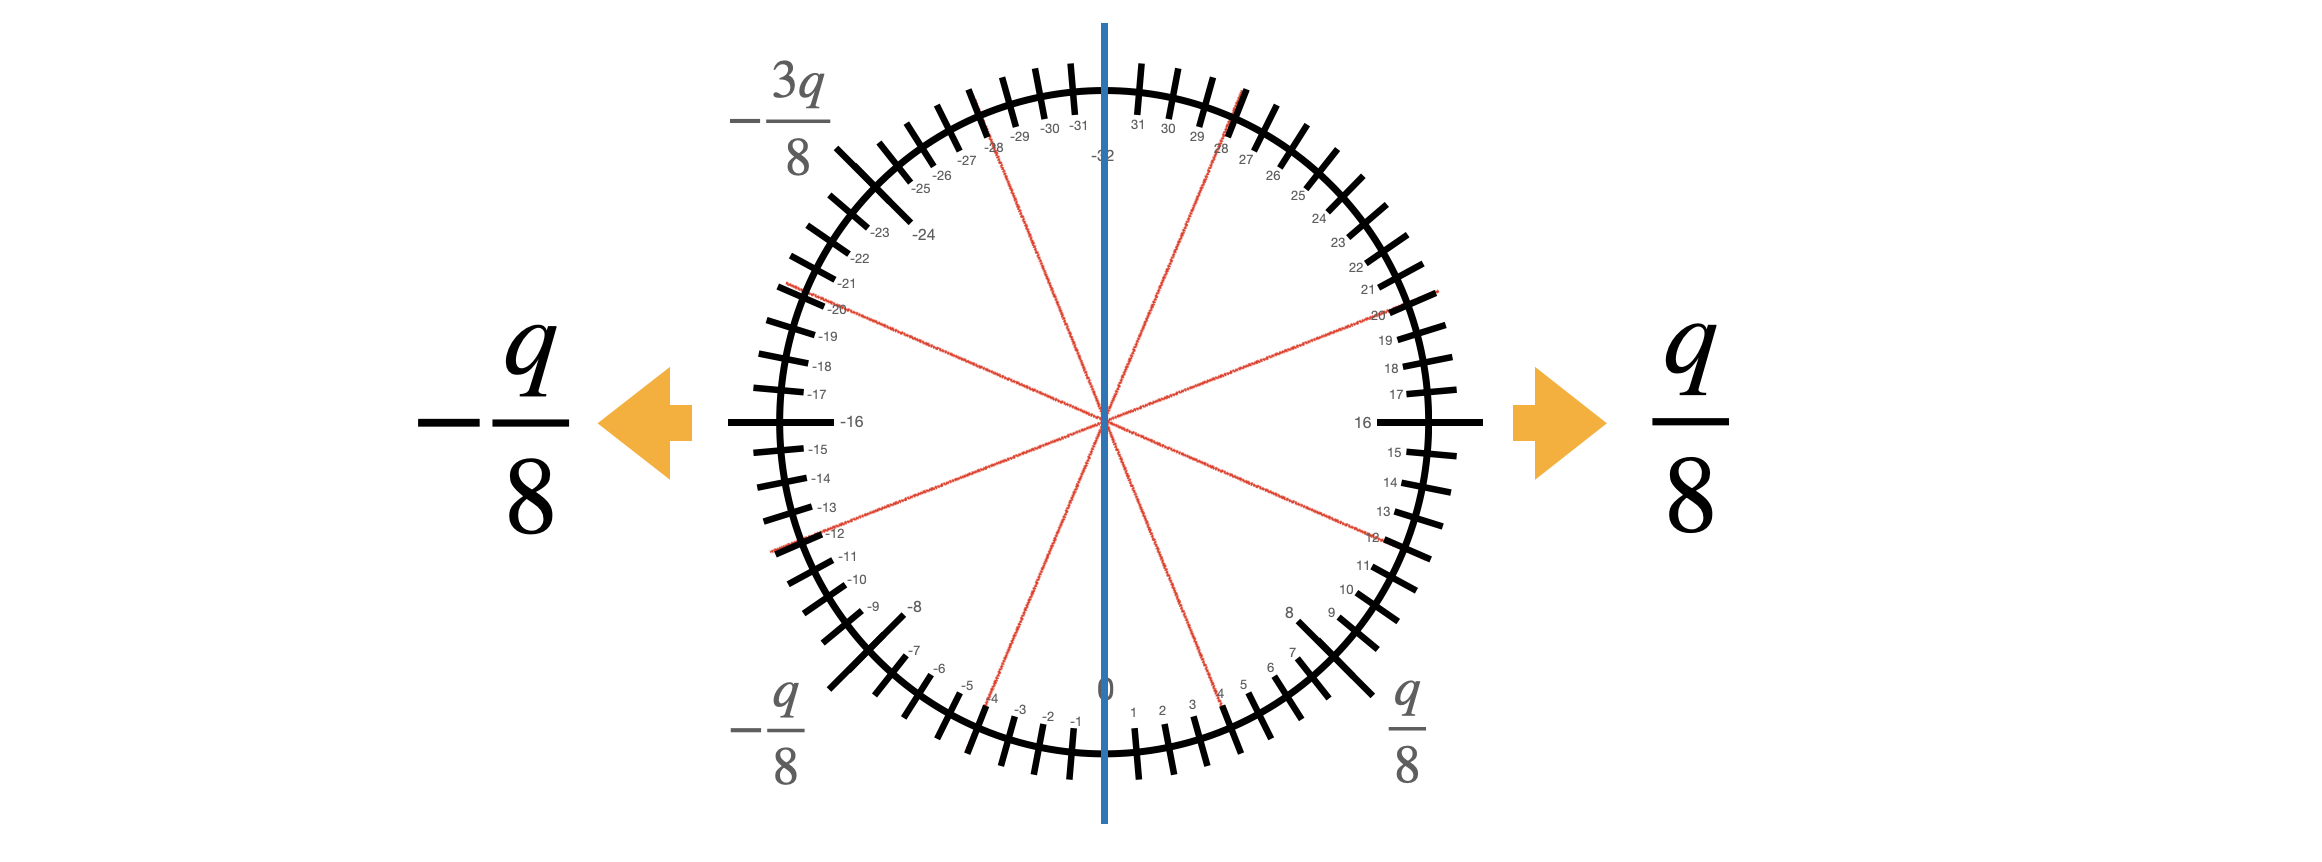
\includegraphics[width=\linewidth]{figures/torus-gate.png}
%  \caption{An illustration of an AND gate in Torus \href{https://assets-global.website-files.com/622ef9de9152c97467eac748/6298a348a0c75850f0688c83_NAND_bootstrap.png}{(Source)}}
%  \label{fig:torus-gate}
%\end{figure}


\autoref{tab:gate-and} is a programmable bootstrapping design for an AND logic gate. For this application, we define the LUT polynomial $V$ as $V(X) = \sum\limits_{i=0}^{7}-X^i$. The LUT polynomial $V(X)$ maps one half of the plaintext domain to $-1$, while the other half to $-1$ (as the terms wrap around the boundary of $n=7$). In this design setup, each bit is separately encrypted as independent TFHE ciphertext. Gate input 0 and 1 are encoded as $-1$ and $1$, respectively. The linear combination (i.e., homomorphic computation formula) for an AND gate is $\textsf{LWE}_{\vec{s}, \sigma}(\Delta m_1) + \textsf{LWE}_{\vec{s}, \sigma}(\Delta m_2) - 1$. Its output is positive if both inputs are positive (i.e. $1$, in which case the blind rotation will rotate $V$ to the left by $\hat\Delta\cdot 1 + e$ positions and the constant term's coefficient will be $1$. Thus, the output of blind rotation and coefficient extraction will be $\textsf{LWE}_{\vec{s}, \sigma}(\Delta \cdot 1)$ with a reduced noise, which is an encoding of $1$. This design can tolerate the maximum noise of $|e| = 1$. To endure bigger noises, we should increase $q$ and $n$. 

Note that the AND gate's LUT layout is negacyclic, which is a special case, thus we could use the entire $2n=16$ coefficient states in $V(X)$ for the AND gate mapping function's outputs, by leveraging $V(X)$'s innate property of negacyclic rotation. However, in many use cases, the LUT layout is not necessarily negacyclic like this AND gate example. Even our noise bootstrapping's LUT layout (\autoref{subsec:bootstrapping-overview}) was not negacyclic, but a unity function (as it simply removes the noise). Thus, for most use cases, we need to use only $\dfrac{t}{2}$ out of $t$ plaintext space to avoid more than $n-1$ rotations of $V(X)$ (\autoref{subsec:tfhe-zero-padding}). 

Besides the AND gate, other logic gates can be built in a similar manner, each of which based on a different linear combination formula and LUT layout. 

\para{Division:} TFHE does not support direct division of plaintext numbers of any size. This is because TFHE's LWE vector elements are in the $Z_q$ ring, where each element $g$ does not necessarily have a multiplicative inverse $g^{-1}$, which makes it hard to multiply $g^{-1}$ to the target number to divide. Instead, division can be implemented as binary division based on the gates implemented by gate bootstrapping. To support binary division, each plaintext has to be a single bit and encrypted as an independent ciphertext. Or multiple bits can be bundled up and processed concurrently by designing a linear combination formula, similar to the linear combination that we designed for processing 2 input bits of an AND gate.

\subsubsection{Application: Neural Networks Bootstrapping}
\label{subsec:tfhe-neural-network}

\begin{figure}[h!]
    \centering
  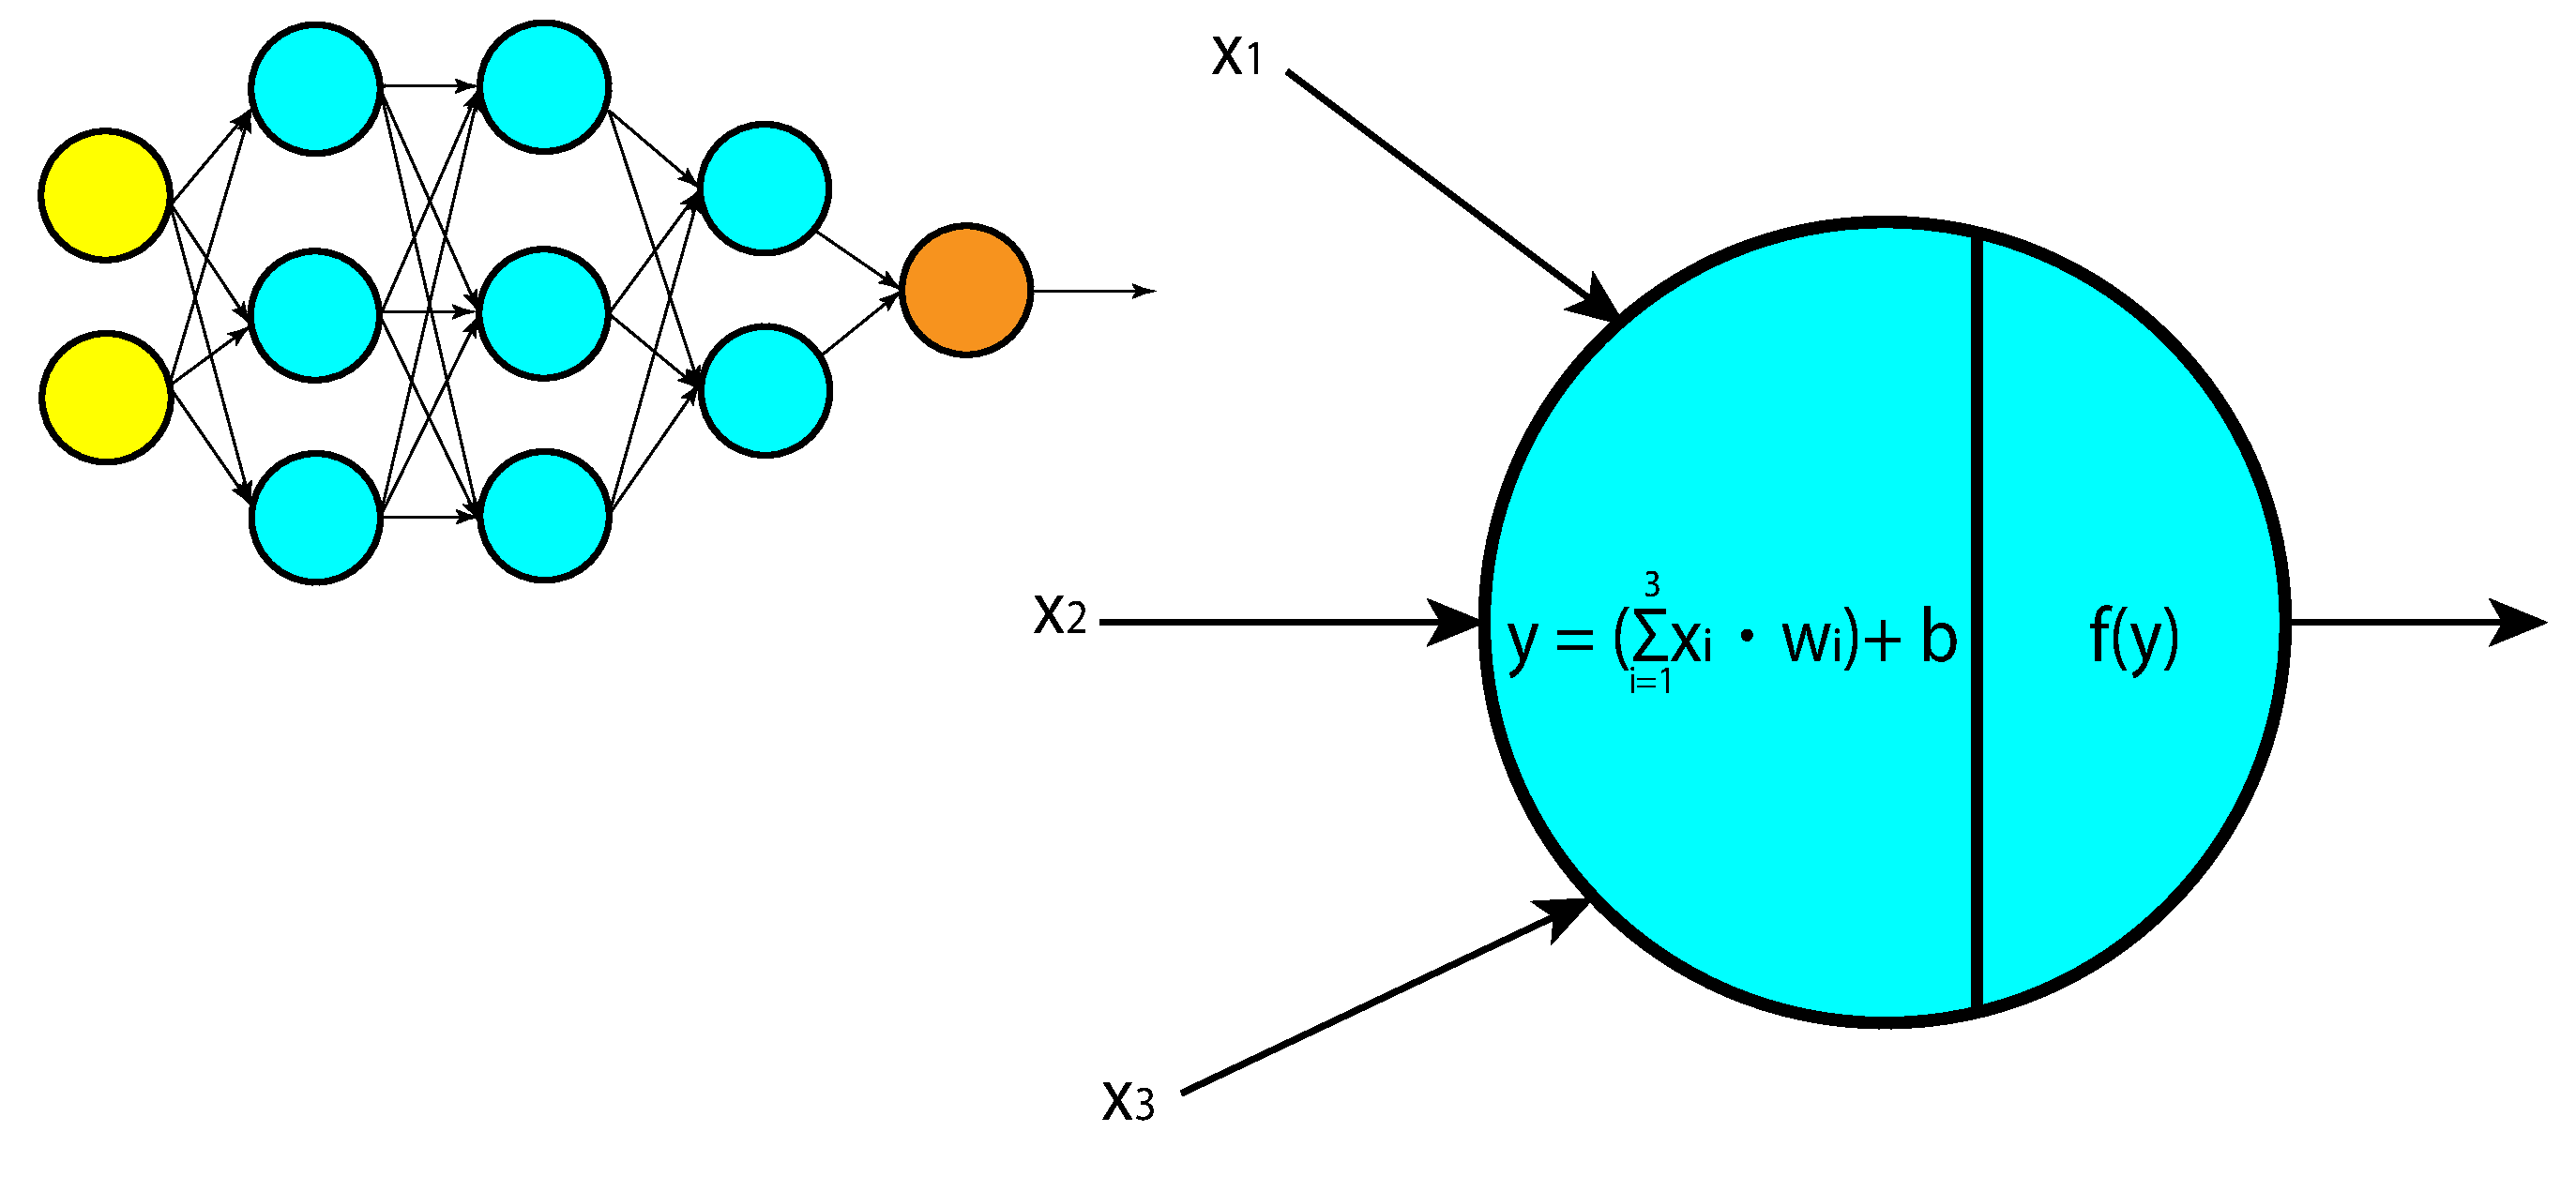
\includegraphics[width=0.8\linewidth]{figures/neural-network.pdf}
  \caption{An illustration of neural networks }
  \label{fig:neural-network}
\end{figure}

\begin{figure}[h!]
    \centering
  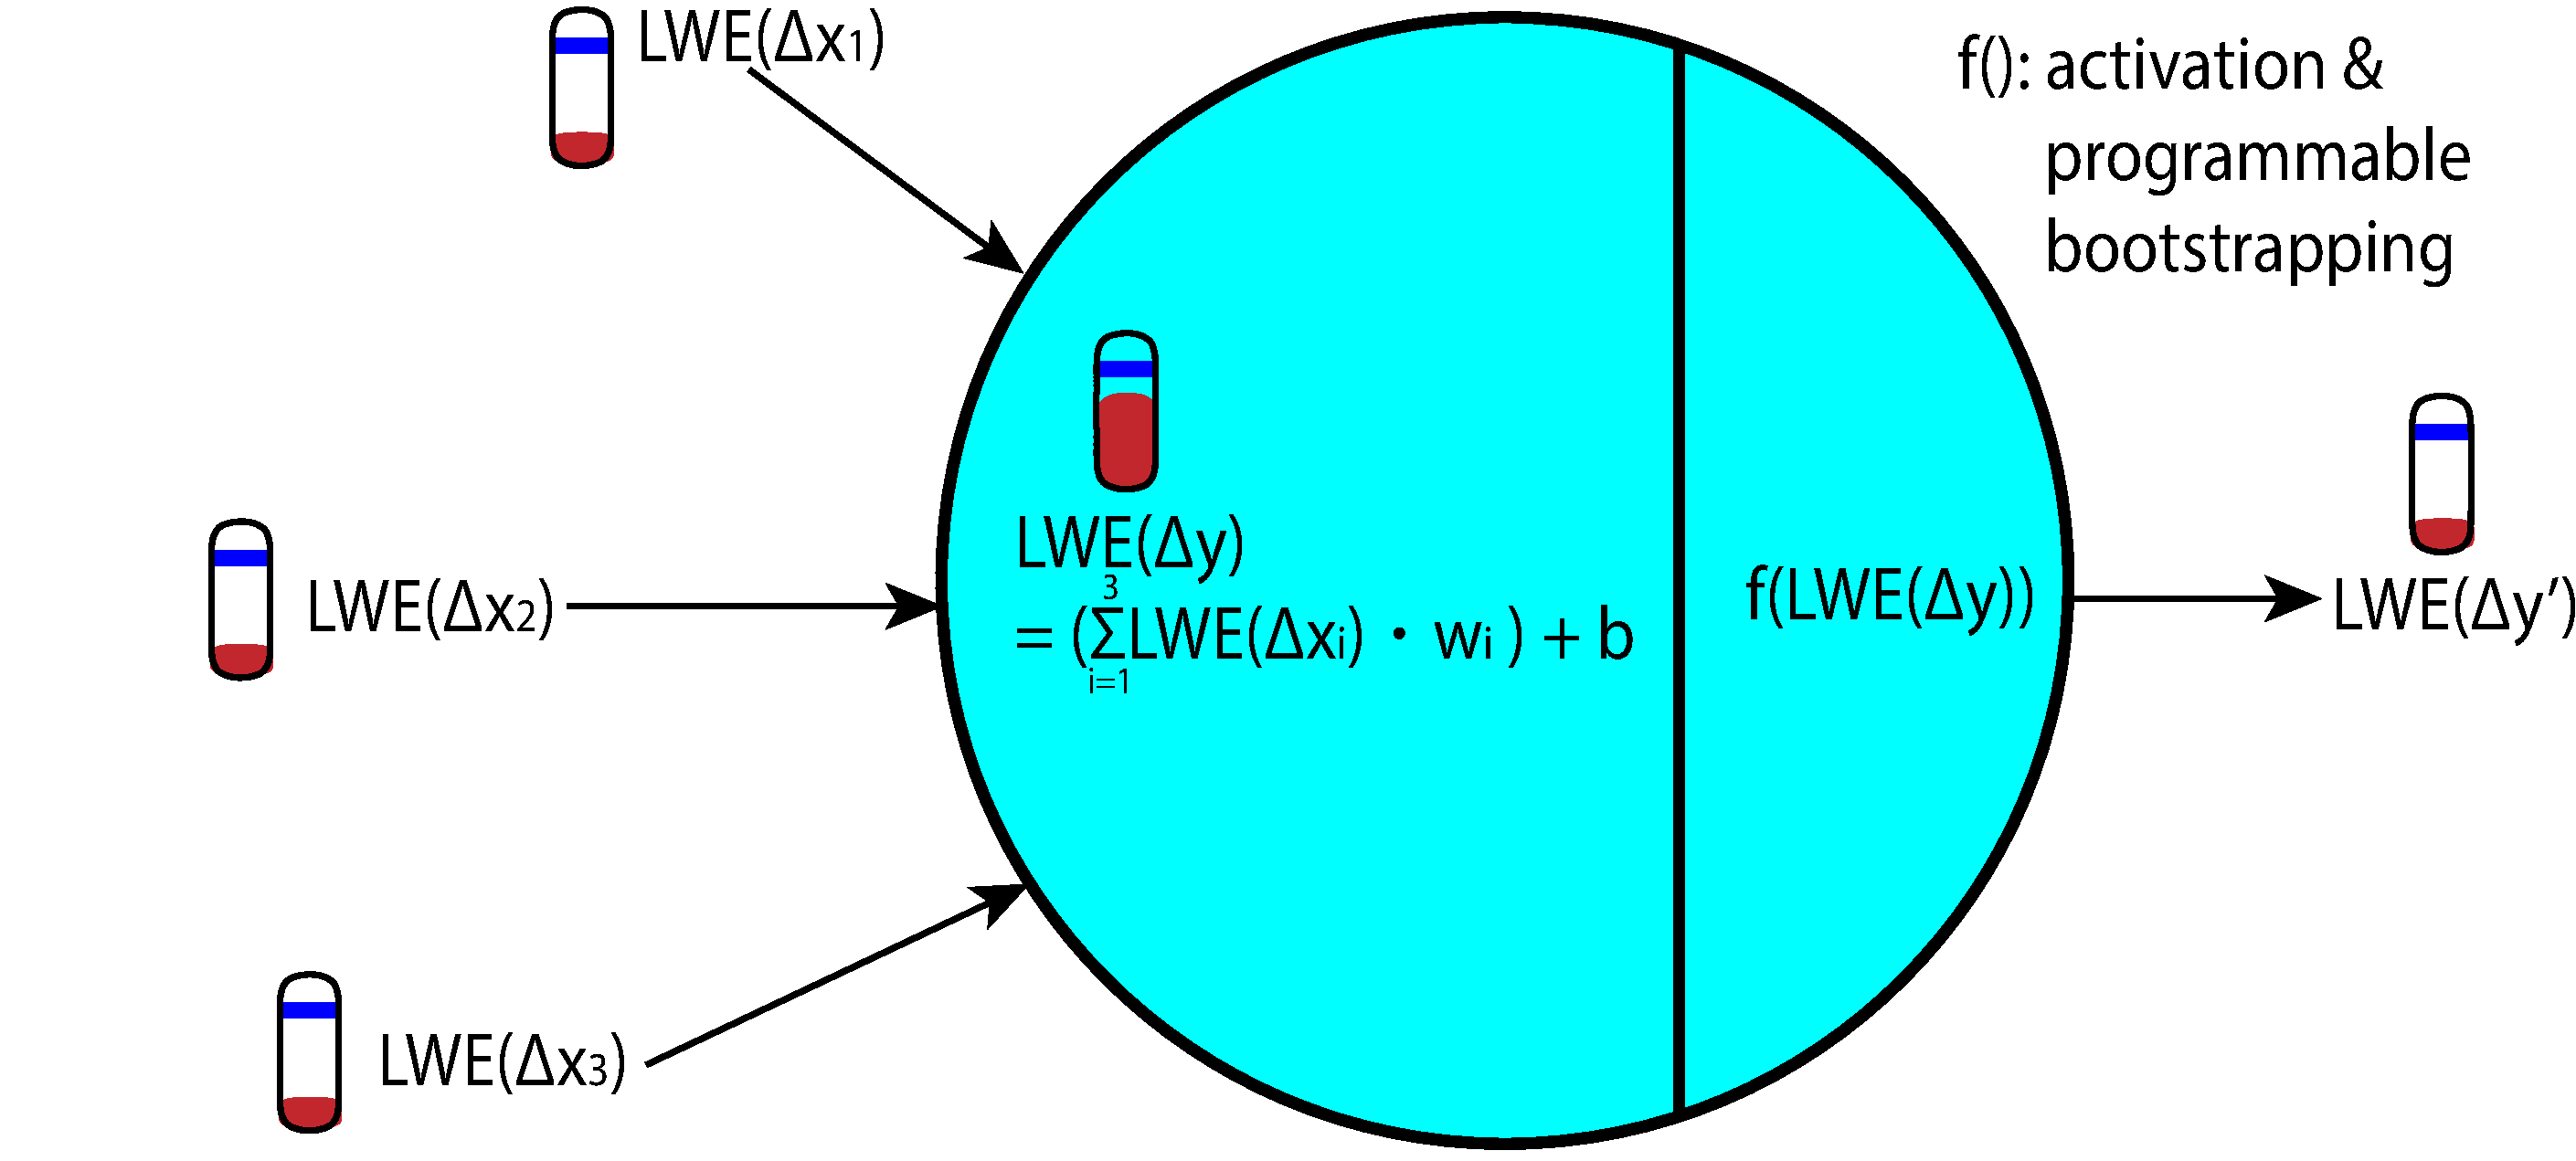
\includegraphics[width=0.8\linewidth]{figures/nn-homomorphic.pdf}
  \caption{An illustration of neural networks's programmable bootstrapping}
  \label{fig:neural-network2}
\end{figure}

Homomorphic encryption can be applied to the neurons of deep neural networks, in which each neuron is generally comprised of two steps of computation: 

\begin{enumerate}
\item \textbf{Linear Combination of Input Values:} An input feature value (or intermediate value) set $(x_1, x_2, \gap{$\cdots$}, x_n)$, a weight set $(w_1, w_2, \gap{$\cdots x$}, w_n)$, and a bias $b$ are computed as: $y = \sum\limits_{i=1}^{n}a_0w_0 + b$. 
\item \textbf{Activation Function:} $f(y)$ is computed, where $f$ is a non-linear activation function such as the $\sin$ function, ReLU, sigmoid, hyperbolic tangent, etc. 
\end{enumerate}

TFHE can homomorphically compute the 1st step's linear combination formula: $y = \sum\limits_{i=1}^{n}a_0w_0 + b$ as $\sum\limits_{i=1}^{n}\textsf{LWE}_{\vec{s}, \sigma}(a_0) \cdot w_0 + b$, which can be implemented as ciphertext addition (\autoref{sec:glwe-add-cipher}) and ciphertext-to-plaintext multiplication (\autoref{sec:glwe-mult-plain}). 

However, the 2nd step's non-linear functions cannot be expressed as addition and multiplication of ciphertexts. To address this issue, the activation function can be evaluated as a programmable bootstrapping, such that the output of the bootstrapping matches or (or is similar) to the output of the activation function. If we use bootstrapping at the 2nd step, noises can be refreshed at the end of every neuron, thus we can potentially handle neural networks of any depth without worrying about the noise growth.



\subsection{TFHE on a Discrete Torus}
\label{subsec:torus}

\textbf{- Reference:} 
\href{https://eprint.iacr.org/2021/1402.pdf}{Guide to
Fully Homomorphic Encryption
over the [Discretized] Torus}~\cite{torus}

$ $

Torus $\mathbb{T}$ is a continuous real number domain between 0 and 1 that wraps around, that is $[0, 1)$. 

A discrete torus $\mathbb{T}_t$ is a finite real number set: $\Big(0, \dfrac{1}{t}, \dfrac{2}{t}, \gap{$\cdots$}, \dfrac{t - 1}{t}\Big)$


In the previous subsections, we explained the TFHE scheme based on the following setup:

$ $

$m \in \mathbb{Z}_t$ 
$\vec{s} = \{0, 1\}^{k}$
$e \in \mathbb{Z}_q$

$\textsf{LWE}_{\vec{s}, \sigma}(\Delta m) = (a_0, a_1, \gap{$\cdots$}, a_k, b) \in \mathbb{Z}_t^{k + 1}$

$ $

However, the original TFHE scheme is designed based on a discrete torus:


$ $

$m \in \mathbb{T}_{t}, \text{ } \vec{s} \in \{0, 1\}^{k}, \text{ } e \in \mathbb{T}_{q}$

$ $

$\textsf{LWE}_{\vec{s}, \sigma}(m) = \textsf{ct} = (a_0, a_1, \gap{$\cdots$}, a_k, b) \in \mathbb{T}_{q}^{k+1}$

$b = \sum\limits_{i=0}^{k}(a_is_i) + m + e \in \mathbb{T}_q$

$\textsf{LWE}_{\vec{s}, \sigma}^{-1}(\textsf{ct}) =  \Big\lceil b - \sum\limits_{i=0}^{k-1}(a_is_i) \Big\rfloor_{\frac{1}{t}} = \Big\lceil m + e \Big\rfloor_{\frac{1}{t}} = m$, given $e < \dfrac{1}{2t}$  

\textcolor{red}{\# where $\lceil x \rfloor_{\frac{1}{t}}$ means rounding $x$ to the nearest multiple of $\dfrac{1}{t}$}

$ $

The original TFHE's difference is that all values (either polynomial coefficients or vector elements) are computed in a floating point modulo 1 (i.e., $[0, 1)$) instead of a big integer (i.e., $[0, q)$). This means the plaintext also has to be encoded as values within $[0, 1)$ instead of integers within $[0, q)$. Note that in the original TFHE scheme, there is no need of the scaling factor $\Delta$, because the continuous domain of torus $[0, 1)$ provides a floating-point precision up to $q$ discrete decimal values, and its decryption process can successfully blow away the noise $E$ as far as each coefficient (or vector element) $e_i$ in $E$ is smaller than $\dfrac{1}{2t}$. 

Both the torus-based and integer-ring-based TFHE schemes are built based on the same fundamental principles.